\documentclass[12pt,a4paper]{ctexart}

% === 页面设置 ===
\usepackage[margin=2.5cm]{geometry}
\usepackage{graphicx}
\usepackage{amsmath,amssymb}
\usepackage{booktabs}
\usepackage{hyperref}
\usepackage{enumitem}
\usepackage{caption}
\usepackage{subcaption}
\usepackage{fancyhdr}
\usepackage{listings}
\usepackage{xcolor}

\hypersetup{colorlinks=true,linkcolor=blue,urlcolor=blue}
\pagestyle{fancy}
\fancyhf{}
\fancyhead[L]{数学建模方法体系与Python实现}
\fancyhead[R]{\thepage}
\renewcommand{\headrulewidth}{0.4pt}

% === 代码风格 ===
\lstset{
    basicstyle=\ttfamily\small,
    breaklines=true,
    frame=single,
    backgroundcolor=\color{gray!5},
    rulecolor=\color{gray!30}
}

\title{\vspace{-2cm}\textbf{数学建模方法体系与Python实现}\\[4pt]}
\author{卫健康 \quad 谷理想 \quad 石智中}
\date{2026年7月}

\begin{document}

\maketitle

% ============================================================
\begin{abstract}
\noindent 本文系统梳理了数学建模中最常用的十类方法，建立了覆盖\textbf{优化建模}、\textbf{图论算法}、\textbf{微分方程数值解}、\textbf{决策与评价}、\textbf{数据预处理}、\textbf{智能优化}、\textbf{生物种群模型}、\textbf{机器学习预测}、\textbf{计算电磁学}及\textbf{CT图像重建}的方法体系。
针对每个模块，给出了数学模型、关键公式、Python实现代码和可视化结果，形成从理论到实践的闭环，可作为数学建模学习和应用的技术参考。

\textbf{关键词}：数学建模；数值计算；Python；优化算法；图论；微分方程；综合评价
\end{abstract}

% ============================================================
\section{引言}

数学建模是将实际问题转化为数学问题、通过计算求解并分析结果的过程。
面对一个具体的建模问题，核心挑战在于从众多候选方法中选择合适的数学工具——是优化问题还是评价问题？是确定性模型还是随机模型？是连续系统还是离散系统？
这一判断能力建立在方法论的广度之上：了解每类方法的适用场景、数学形式和求解途径，才能在有限时间内做出正确的技术决策。

Python科学计算生态（NumPy、SciPy、Matplotlib、scikit-learn、NetworkX等）为数学建模提供了从数据处理到模型求解到结果可视化的完整工具链。
本文按照专题模块，系统梳理了数学建模中最常用的十类方法——\textbf{优化建模}、\textbf{图论算法}、\textbf{微分方程数值解}、\textbf{决策与评价}、\textbf{插值与拟合}、\textbf{智能优化}、\textbf{生物种群模型}、\textbf{机器学习预测}、\textbf{计算电磁学}及\textbf{CT图像重建}。
每个模块给出数学模型、关键公式、Python实现和可视化结果，各模块的完整可运行代码见配套demo脚本。

% ============================================================
\section{优化方法：从线性规划到整数规划}

优化问题是国赛中最常见的题型之一。无论是生产计划、资源分配，还是物流调度、投资组合，本质都是在一组约束条件下寻找目标函数的最优值。

\subsection{线性规划 (LP)}

线性规划的标准形式为：
\begin{equation}
\begin{aligned}
\min \quad & \mathbf{c}^T \mathbf{x} \\
\text{s.t.} \quad & A\mathbf{x} \leq \mathbf{b},\quad \mathbf{x} \geq 0
\end{aligned}
\end{equation}

以生产计划问题为例：某工厂生产A、B两种产品，A利润40元/件，B利润60元/件。A需1h机器加工+2h人工，B需2h机器加工+1h人工。每天可用机器8h、人工10h。模型如下：
\[
\max\; 40x_1+60x_2,\quad \text{s.t.}\; x_1+2x_2\leq 8,\; 2x_1+x_2\leq 10,\; x_1,x_2\geq 0
\]

使用SciPy的\texttt{linprog}求解，得最优解为$x_1=4$件、$x_2=2$件，最大利润280元，机器和人工利用率均达到100\%。

\subsection{整数规划 (IP) 与0-1规划}

当决策变量必须取整数时（如人数、车辆数、项目选择），需要引入整数约束。0-1整数规划在项目选择、设施选址等场景中尤为常见。

本文实现了投资项目选择的0-1 IP模型（4个项目，资金上限500万，项目1和3互斥），通过枚举法得到最优组合为选择项目1、2、4，总投入450万，总收益185万。同时实现了钢管下料的混合整数规划（MIP）模型，使用SciPy求解后取整修复，得到最少用料方案。

\subsection{求解器选型}

日常建模中，简单LP/NLP使用SciPy即可（无需额外安装），整数规划推荐PuLP+CBC（开源免费），大规模问题可申请Gurobi学术免费版。本文所有demo均基于SciPy+NumPy实现，确保环境依赖最小化。

\begin{figure}[htbp]
\centering
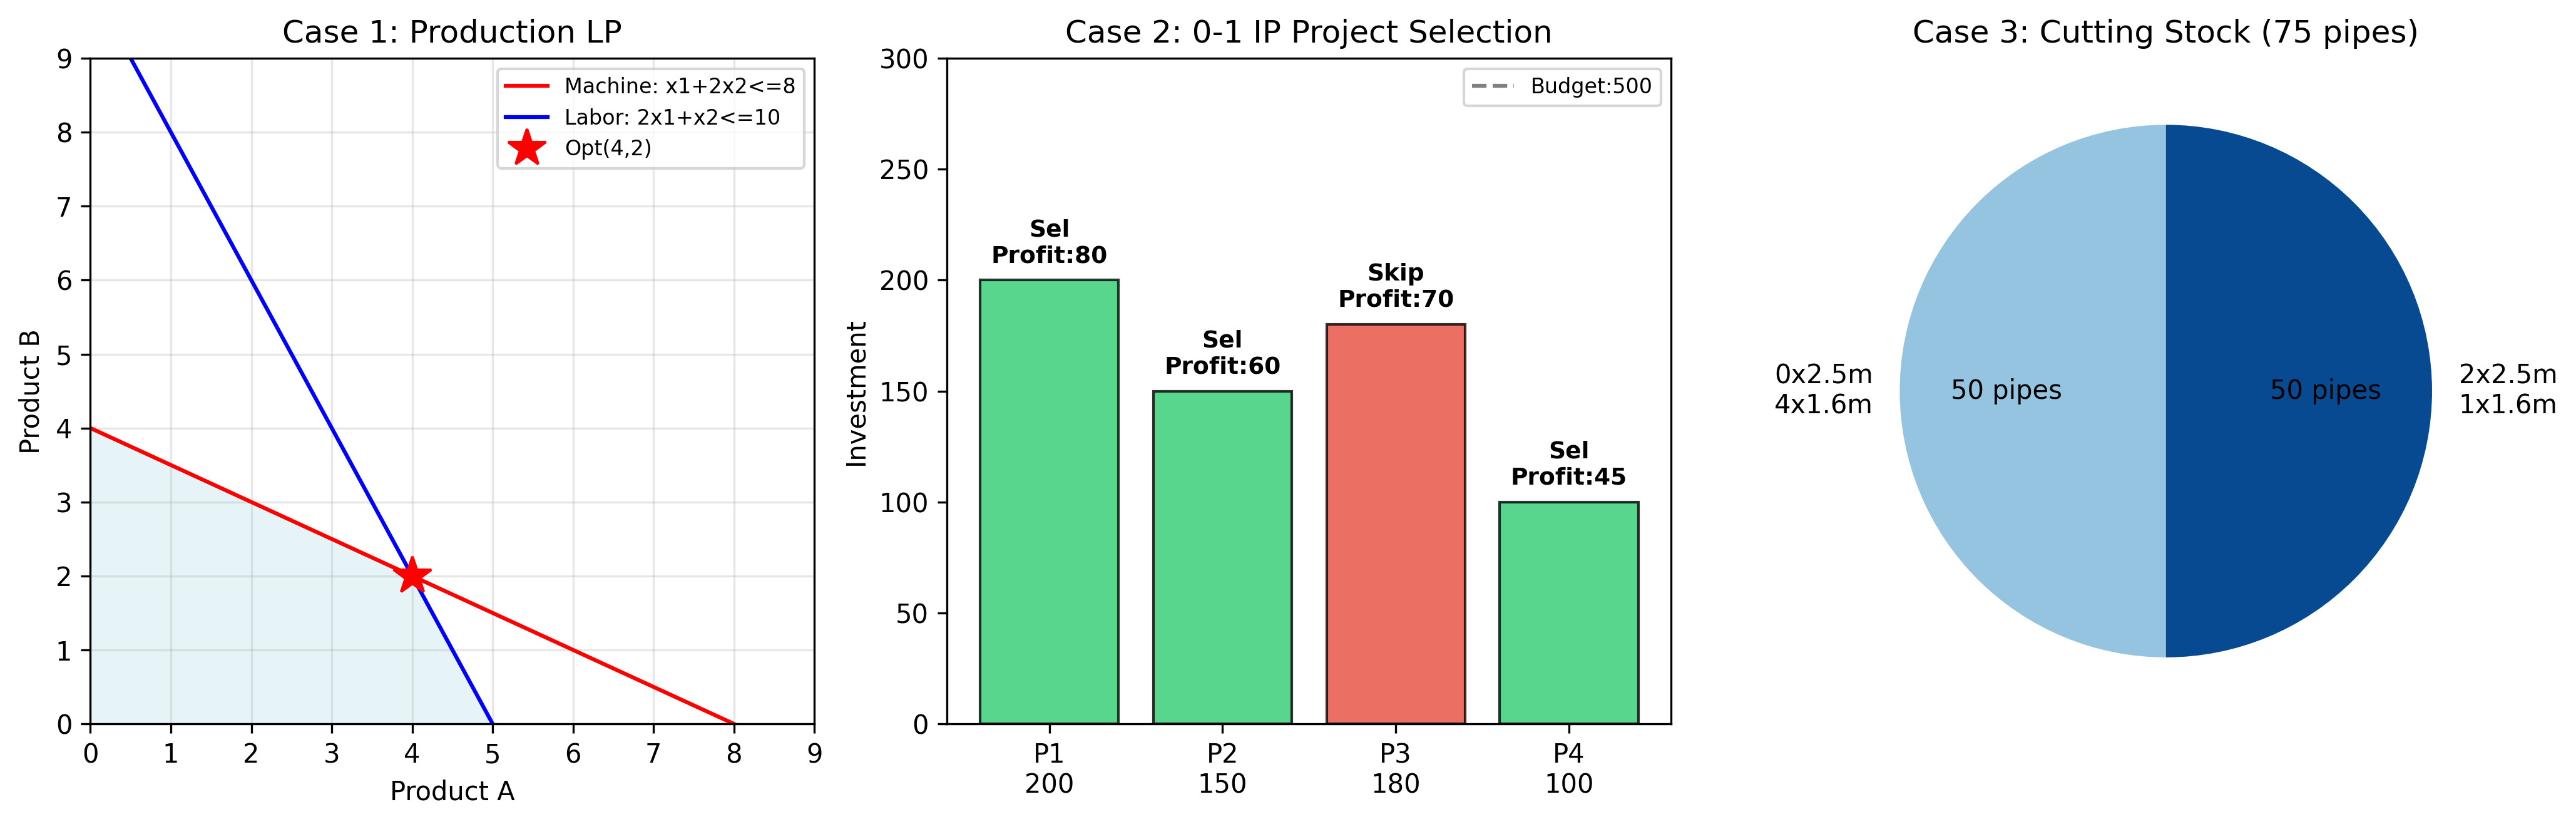
\includegraphics[width=\textwidth]{../output/optimization_result.png}
\caption{优化模型演示：生产计划LP可行域与最优解（左）、0-1投资项目选择（中）、钢管下料方案（右）}
\label{fig:optimization}
\end{figure}

% ============================================================
\section{图论建模：从网络到连通性}

图建模的核心思想是将实际问题抽象为``节点+边''的结构，然后调用成熟的图论算法求解。这一方法论适用于交通网络、物流配送、社交关系、任务调度、通信布线等多种场景。

\subsection{经典算法与应用}

本文实现了四类核心图算法：
\begin{enumerate}[label=(\arabic*)]
    \item \textbf{最短路径 (Dijkstra)}：物资配送网络（7节点、12条边），求得中心到各点的最短路线。
    \item \textbf{最小生成树 (Kruskal)}：6个村庄光纤布线方案，MST总成本31单位。
    \item \textbf{最大流 (Dinic)}：城市供水管网（6节点、9条管道），最大供水量35~m$^3$/h，并给出各管段实际流量分配。
    \item \textbf{二分图匹配 (Hopcroft-Karp)}：4人-4任务分配，实现完美匹配（4对）。
\end{enumerate}

所有图算法均使用NetworkX库实现，该库提供了从建图到求解到可视化的完整API，是数模编程中处理图问题的首选工具。

\subsection{图建模的判断}

当题目中出现``路径、网络、连通、配送、遍历、选址、调度、依赖、管道、布线''等关键词时，应首先考虑是否可以抽象为图模型。图建模与数学规划并非互斥——很多问题可以同时用两种方法求解，形成互补验证，这在论文中是加分项。

\begin{figure}[htbp]
\centering
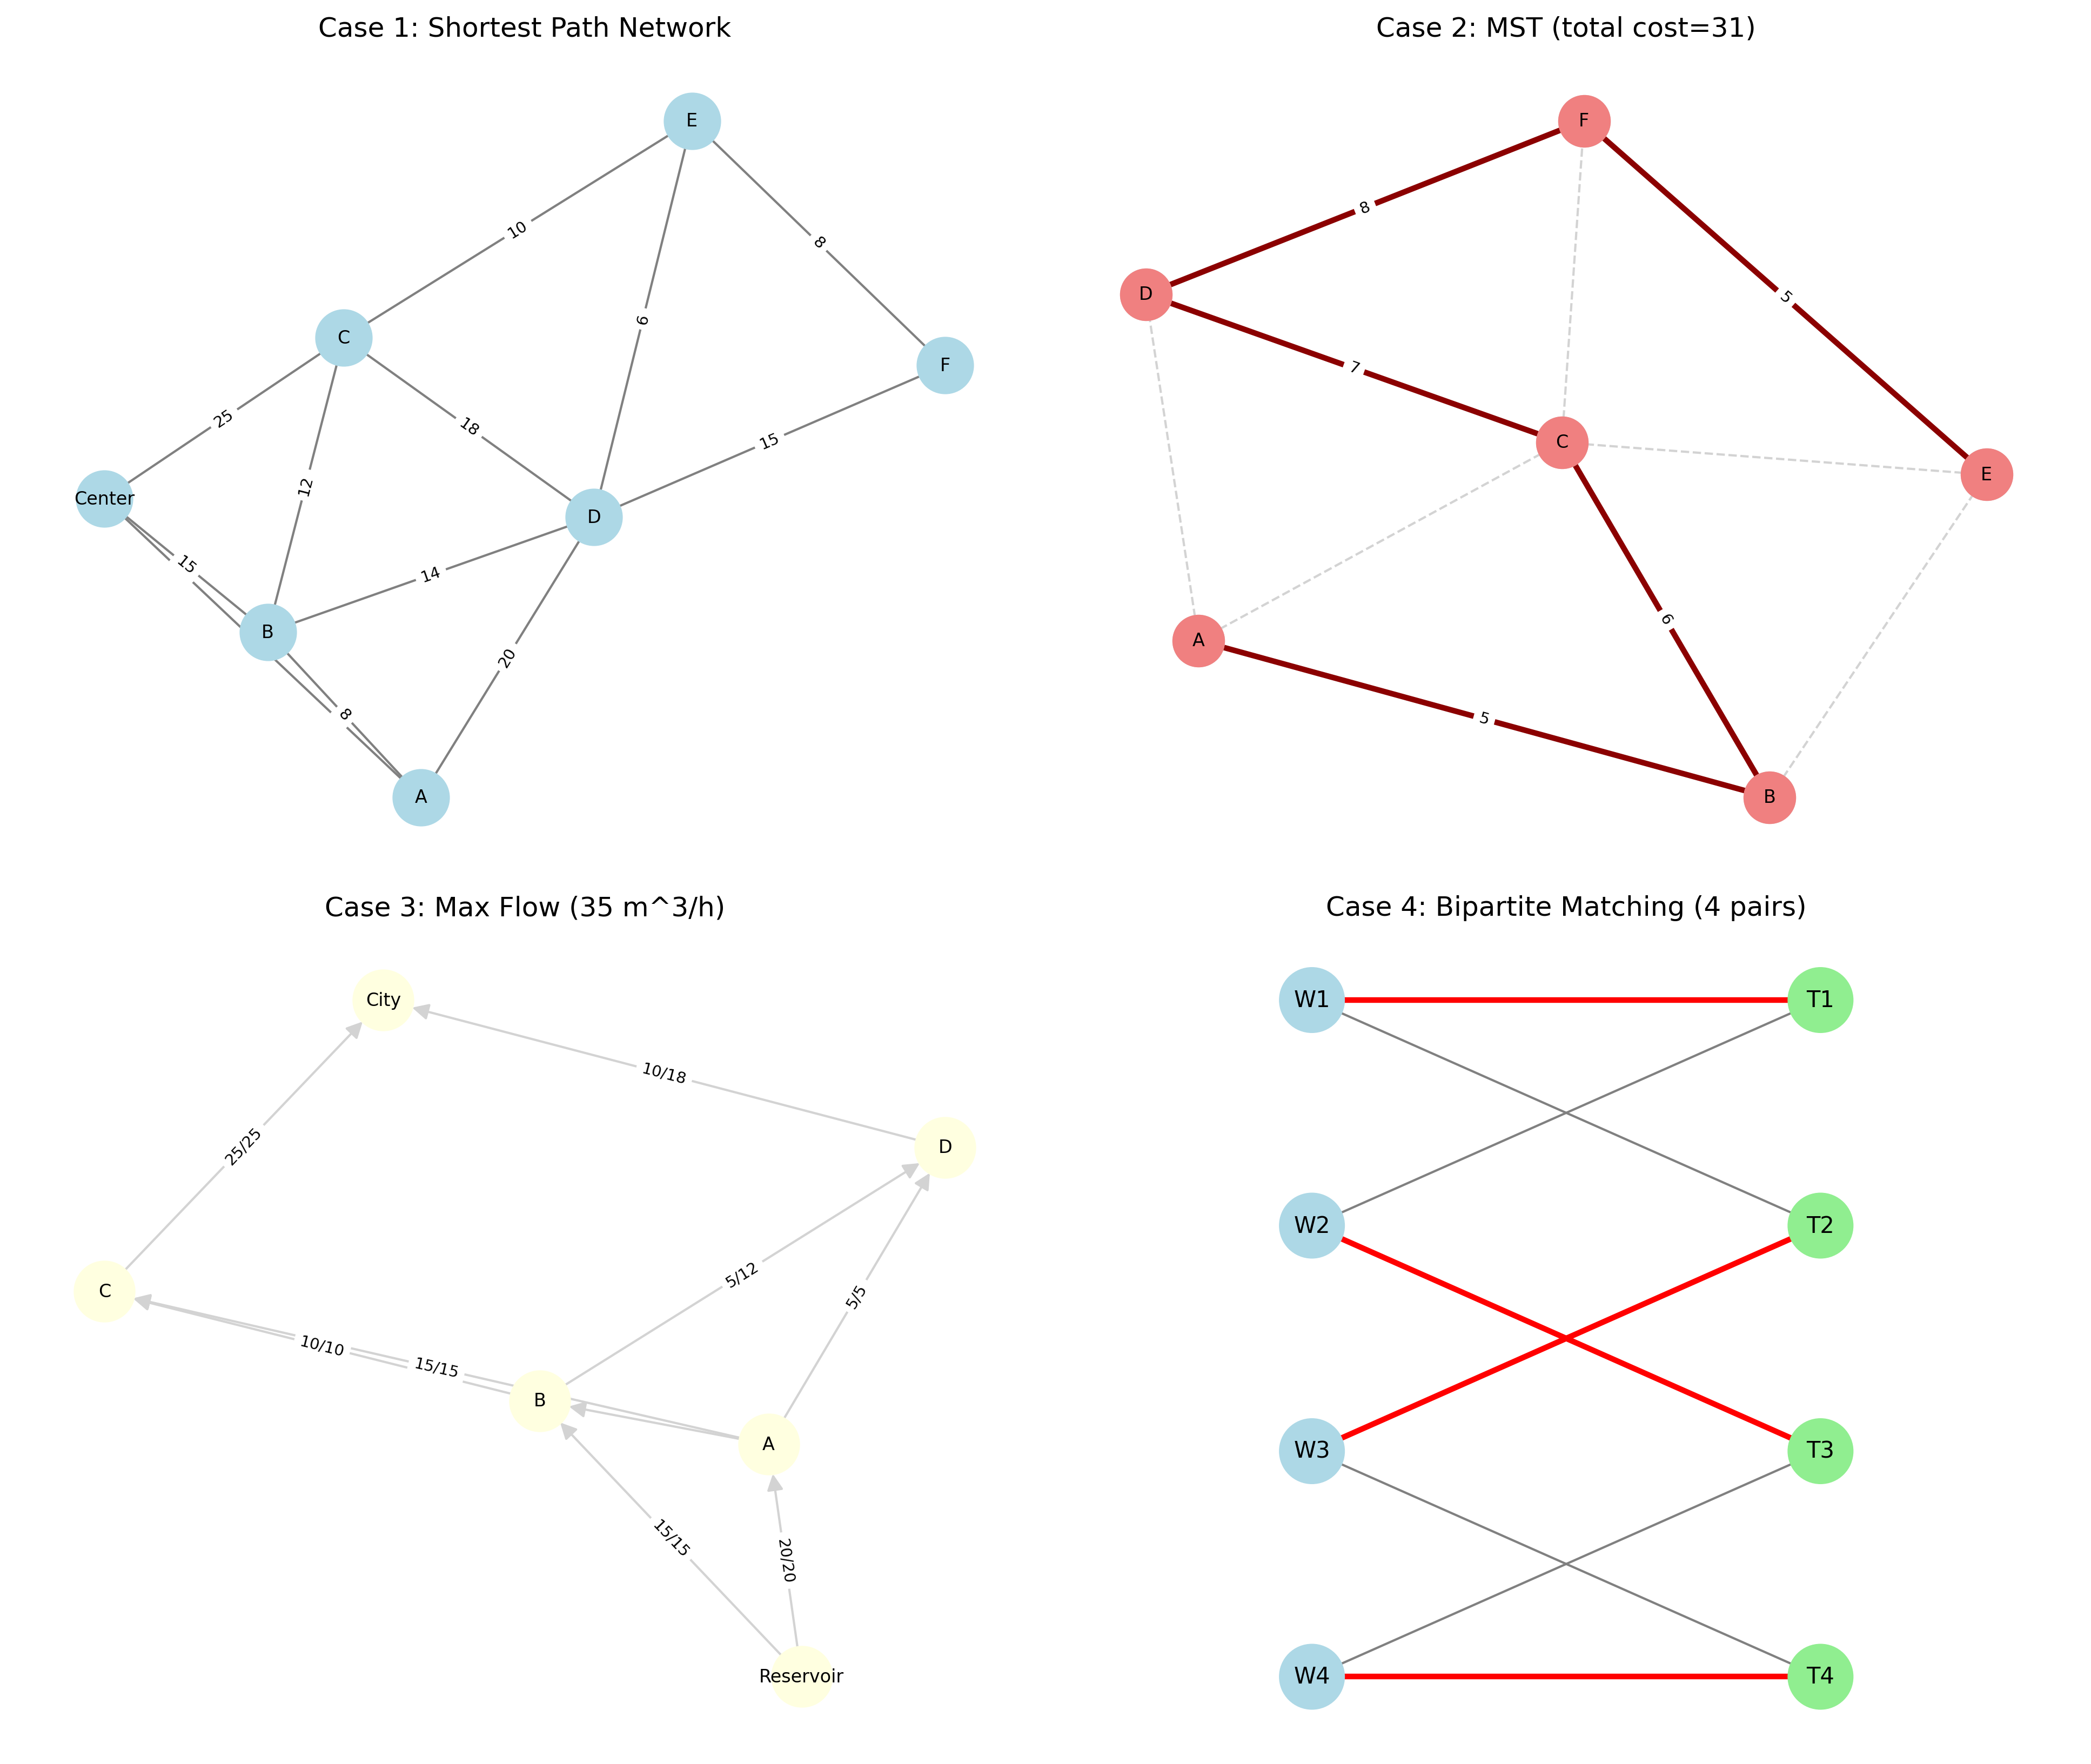
\includegraphics[width=\textwidth]{../output/graph_result.png}
\caption{图论算法演示：最短路径网络（左上）、MST最小生成树（右上）、最大流供水管网（左下）、二分图匹配（右下）}
\label{fig:graph}
\end{figure}

% ============================================================
\section{微分方程数值求解}

微分方程是描述``变化''的数学语言——人口增长、传染病传播、物理运动、化学反应等随时间演化的过程，都需要微分方程来描述。

\subsection{常微分方程 (ODE) 数值方法}

绝大多数实际ODE没有解析解，必须依赖数值方法。SciPy的\texttt{solve\_ivp}是求解ODE初值问题的核心工具。日常使用推荐RK45方法（Dormand-Prince 5(4)阶自适应步长），遇到刚性方程（系统各分量变化速率差异极大）时切换至BDF方法。

本文选取三个经典模型进行了数值求解：
\begin{enumerate}[label=(\arabic*)]
    \item \textbf{SIR传染病模型}：$\frac{dS}{dt}=-\beta\frac{SI}{N},\; \frac{dI}{dt}=\beta\frac{SI}{N}-\gamma I,\; \frac{dR}{dt}=\gamma I$。取$N=10000$、$\beta=0.3$、$\gamma=0.1$，基本再生数$R_0=3.0$，感染峰值出现在第38天（3007人），最终94.0\%人口被感染。
    \item \textbf{Lotka-Volterra捕食者-猎物模型}：$\frac{dx}{dt}=\alpha x-\beta xy,\; \frac{dy}{dt}=\delta xy-\gamma y$。猎物均值25.1，捕食者均值10.0，呈现周期振荡。
    \item \textbf{阻尼振动（二阶ODE降阶法）}：$x''+0.5x'+5x=0$，通过令$v=x'$将二阶方程化为一阶方程组，使用RK45求解504步。
\end{enumerate}

\subsection{偏微分方程 (PDE)}

PDE的数值方法主要包括有限差分法(FDM)、有限元法(FEM)和有限体积法(FVM)。本文以一维热传导方程为例，演示了显式有限差分格式的实现——稳定性条件是$\alpha\Delta t/\Delta x^2<0.5$，这是显式格式的关键约束。

\begin{figure}[htbp]
\centering
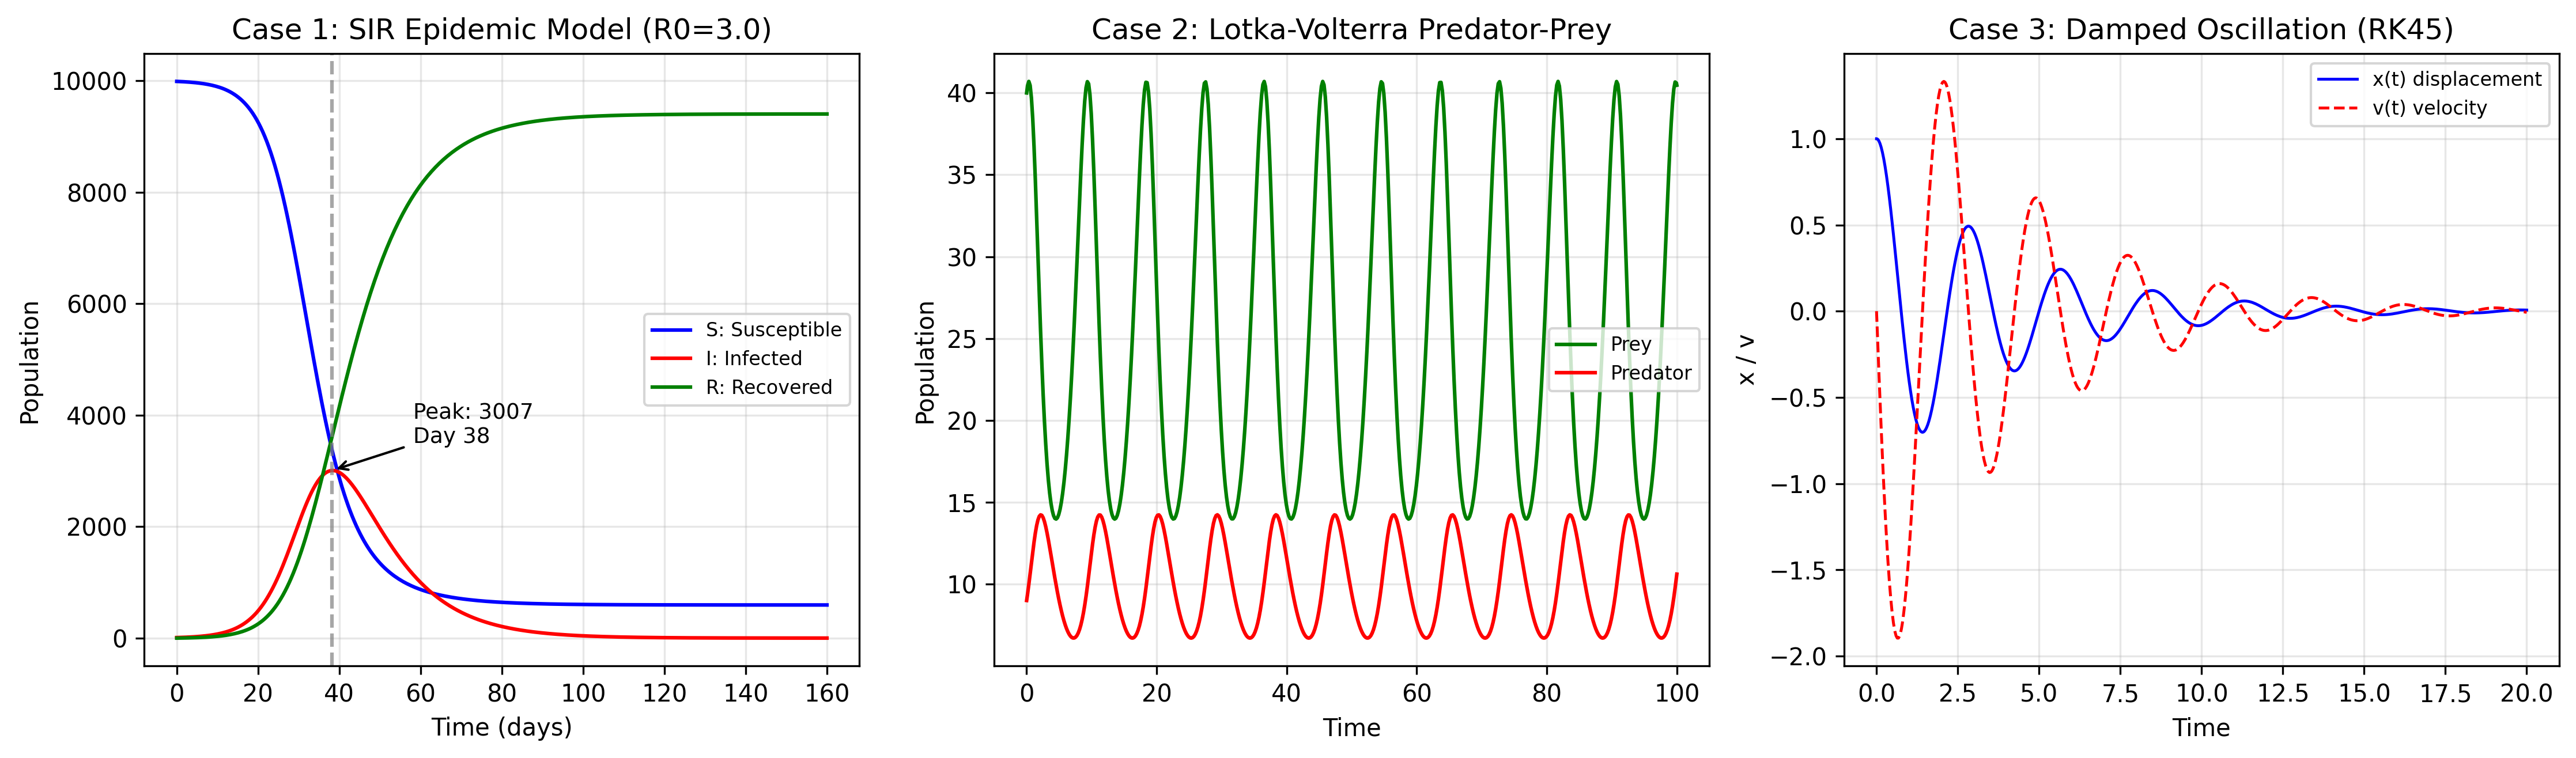
\includegraphics[width=\textwidth]{../output/ode_result.png}
\caption{微分方程数值求解：SIR传染病模型（左）、Lotka-Volterra捕食者-猎物（中）、阻尼振动（右）}
\label{fig:ode}
\end{figure}

% ============================================================
\section{决策与评价模型}

评价与决策问题是国赛的另一大类题型，核心是在多个备选方案中，基于多维指标选出最优方案。

\subsection{层次分析法 (AHP)}

AHP通过将决策问题分解为目标层、准则层和方案层，利用Saaty 1-9标度法构造两两比较判断矩阵，计算最大特征值对应的特征向量作为权重，并引入一致性比率CR检验判断矩阵的合理性。

本文以供应商选择为例，建立了成本、质量、时间三项准则的判断矩阵，计算得到权重分别为0.6370、0.2583、0.1047，CR=0.037<0.1，通过一致性检验。

\subsection{TOPSIS综合评价法}

TOPSIS的核心思想是：最优方案应距离正理想解最近、距离负理想解最远。通过数据正向化$\to$向量归一化$\to$计算欧氏距离$\to$求相对贴近度四步，得到各方案的排序得分。

本文以4个供应商在3个指标（成本、质量、时间）下的表现为例，结合AHP权重进行TOPSIS排序，得到S3>S1>S2>S4的优劣顺序。

\subsection{不确定型决策}

当自然状态的概率未知时，需要使用不确定型决策准则。本文实现了五种经典准则——乐观(max-max)、悲观(max-min)、折中(Hurwicz, $\alpha=0.6$)、后悔值(Savage)、等概率(Laplace)——并对含有三种方案、四种市场状态的收益矩阵进行了分析。

\begin{figure}[htbp]
\centering
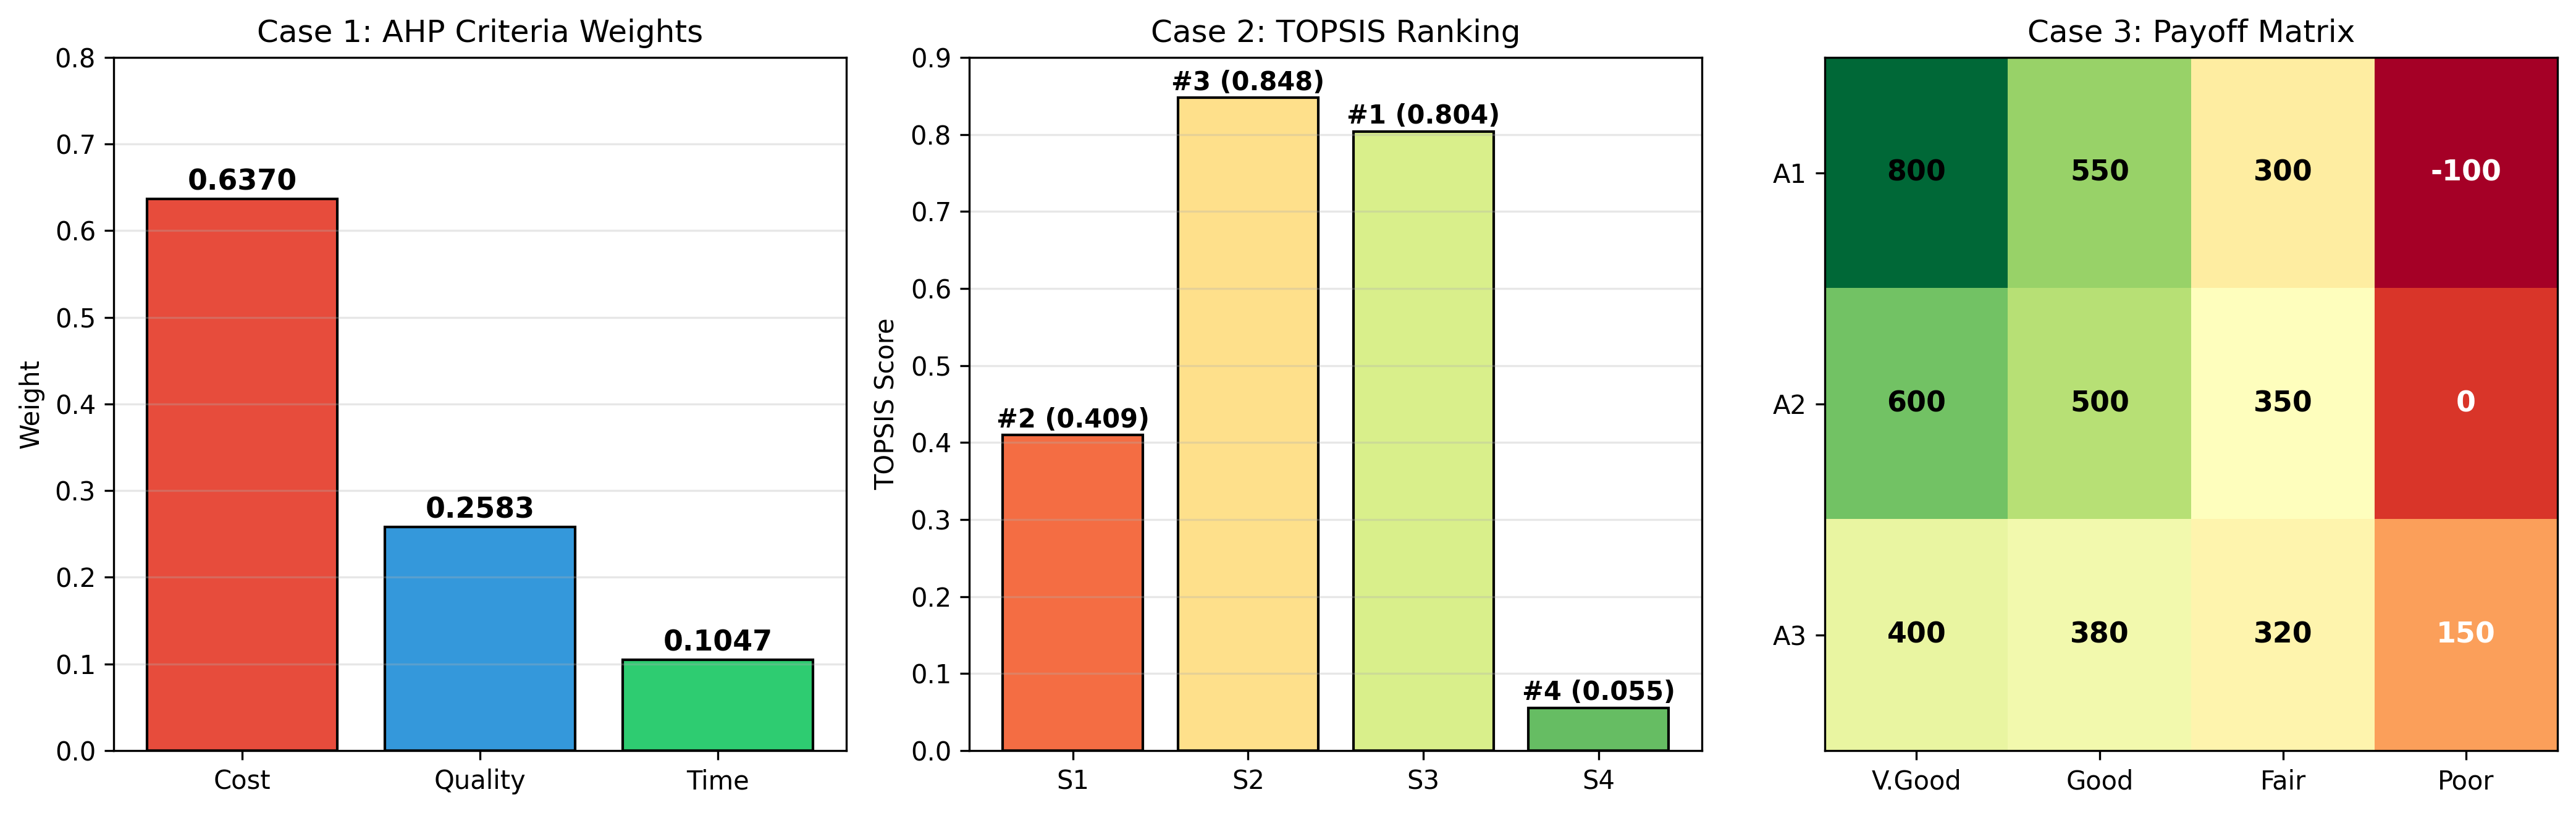
\includegraphics[width=\textwidth]{../output/decision_result.png}
\caption{决策模型演示：AHP准则权重（左）、TOPSIS方案排序（中）、不确定型决策收益矩阵（右）}
\label{fig:decision}
\end{figure}

% ============================================================
\section{数据预处理：插值与拟合}

数据预处理是数学建模的第一步。插值用于从离散数据点估计中间值，拟合用于从含噪声的数据中提取趋势规律。

\subsection{插值方法}

多项式插值面临龙格(Runge)现象——高次多项式在区间端点处会产生剧烈震荡。本文使用$f(x)=1/(1+25x^2)$在$[-1,1]$上演示了这一现象：15次多项式拟合的最大误差达2.11，而4次多项式仅为0.44。解决方案是采用分段低次插值或三次样条插值(\texttt{CubicSpline})，后者在保证光滑性的同时避免了龙格现象。

\subsection{拟合方法}

最小二乘拟合是最常用的数据建模方法。本文演示了多项式拟合（\texttt{numpy.polyfit}）和非线性曲线拟合（\texttt{scipy.optimize.curve\_filt}），并以应力-应变实验数据为例，对比了二次多项式（$R^2=0.9996$）、幂律模型（$R^2=0.157$）和指数偏移模型（$R^2=0.9988$）的拟合效果。

\begin{figure}[htbp]
\centering
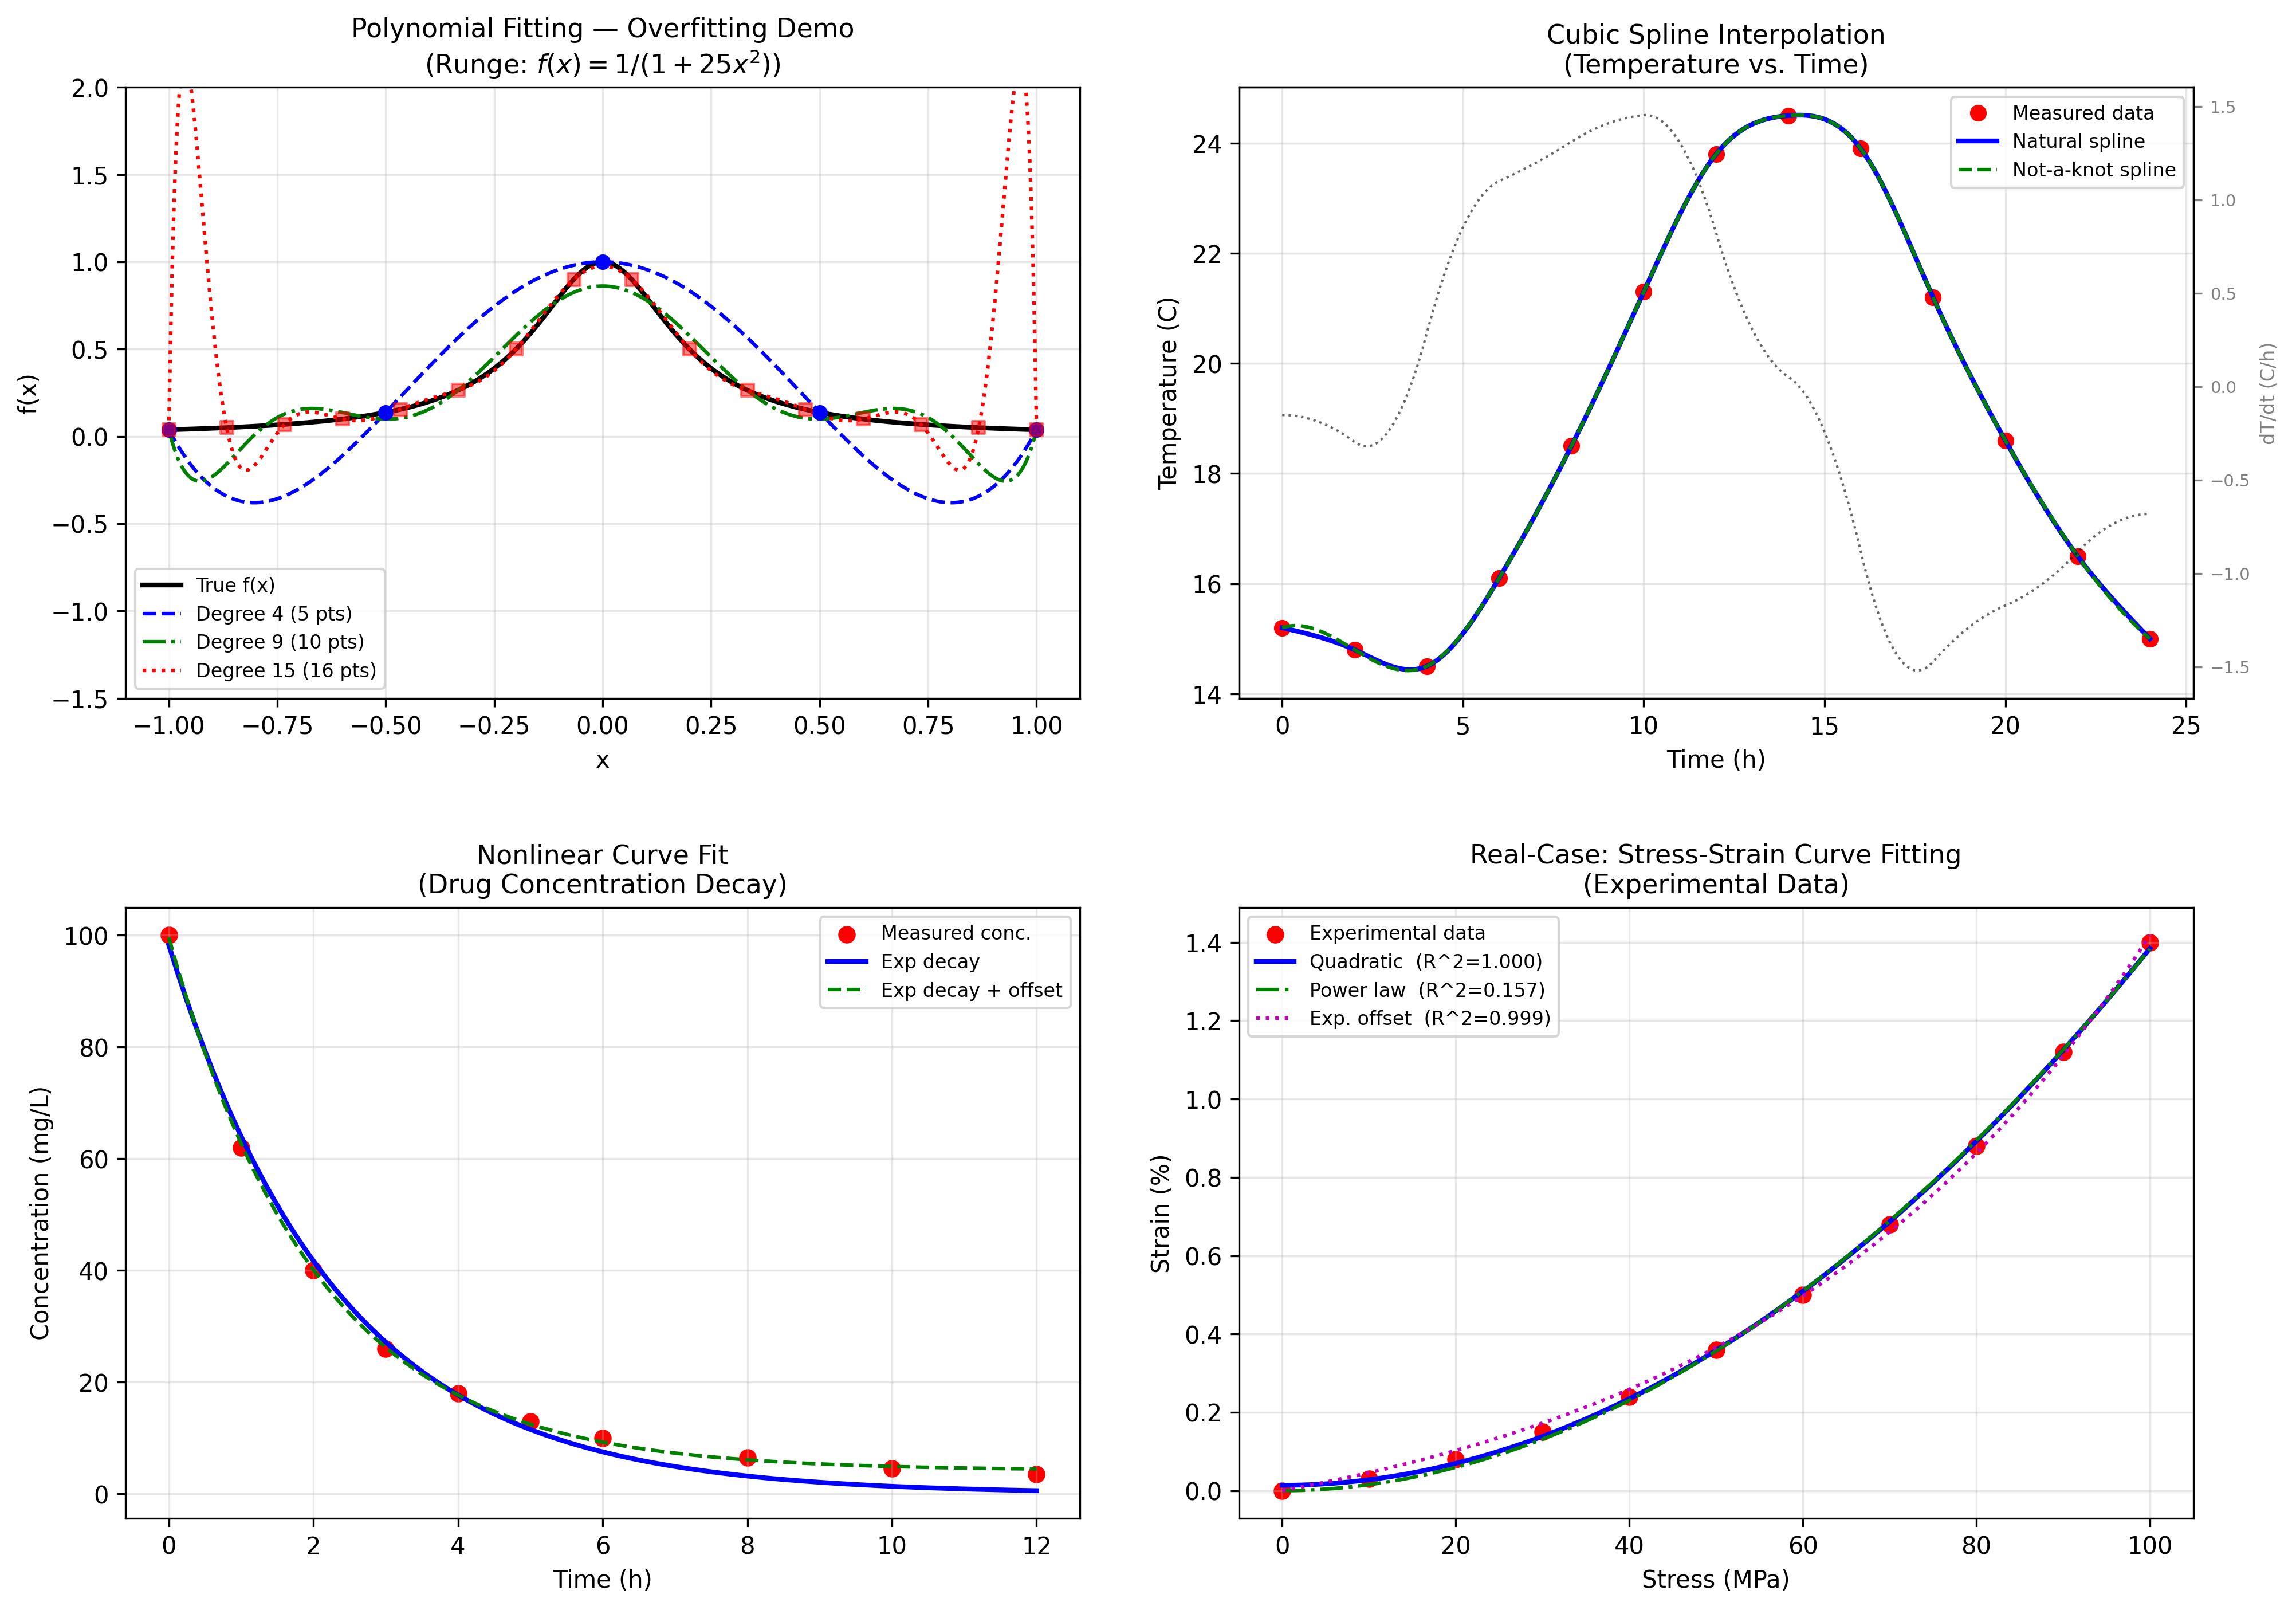
\includegraphics[width=\textwidth]{../output/interpolation_result.png}
\caption{插值与拟合演示：多项式过拟合与龙格现象（左上）、三次样条插值（右上）、非线性curve\_fit（左下）、应力-应变多模型对比（右下）}
\label{fig:interpolation}
\end{figure}

% ============================================================
\section{智能优化算法}

当目标函数不可微、多峰、或问题本身是NP-hard时，传统的梯度优化方法无法使用，需要借助智能优化算法。

\subsection{四种核心算法}

本文手写实现了遗传算法(GA)和粒子群优化(PSO)，并结合SciPy内置函数演示了差分进化(DE)和模拟退火(SA)：

\begin{enumerate}[label=(\arabic*)]
    \item \textbf{遗传算法 (GA)}：模拟自然选择与遗传变异。采用实数编码、SBX交叉、多项式变异、锦标赛选择和精英保留策略，对Sphere函数$f(x)=\sum x_i^2$进行最小化，最终适应度$3.11\times 10^{-6}$（全局最优为0）。
    \item \textbf{粒子群优化 (PSO)}：模拟鸟群觅食行为。采用线性递减惯性权重策略，对Sphere函数求解，最终适应度$3.53\times 10^{-25}$——收敛速度和精度均优于GA。
    \item \textbf{差分进化 (DE)}：使用SciPy的\texttt{differential\_evolution}求解Rastrigin多峰函数，找到精确全局最优$f=0$，仅需1743次函数评估。
    \item \textbf{模拟退火 (SA)}：使用SciPy的\texttt{dual\_annealing}求解Ackley函数，在有限迭代预算下得到$f=2.58$。
\end{enumerate}

\subsection{算法选择策略}

对于实际问题，优先尝试传统优化方法（LP/NLP）。当传统方法失效时，按以下顺序选择：函数可微且单峰$\to$梯度方法；多峰且维度较低$\to$差分进化；离散/组合优化$\to$遗传算法；需要快速收敛$\to$粒子群。智能算法不是万能药——``能用精确方法就不用启发式''是国赛建模的重要原则。

\begin{figure}[htbp]
\centering
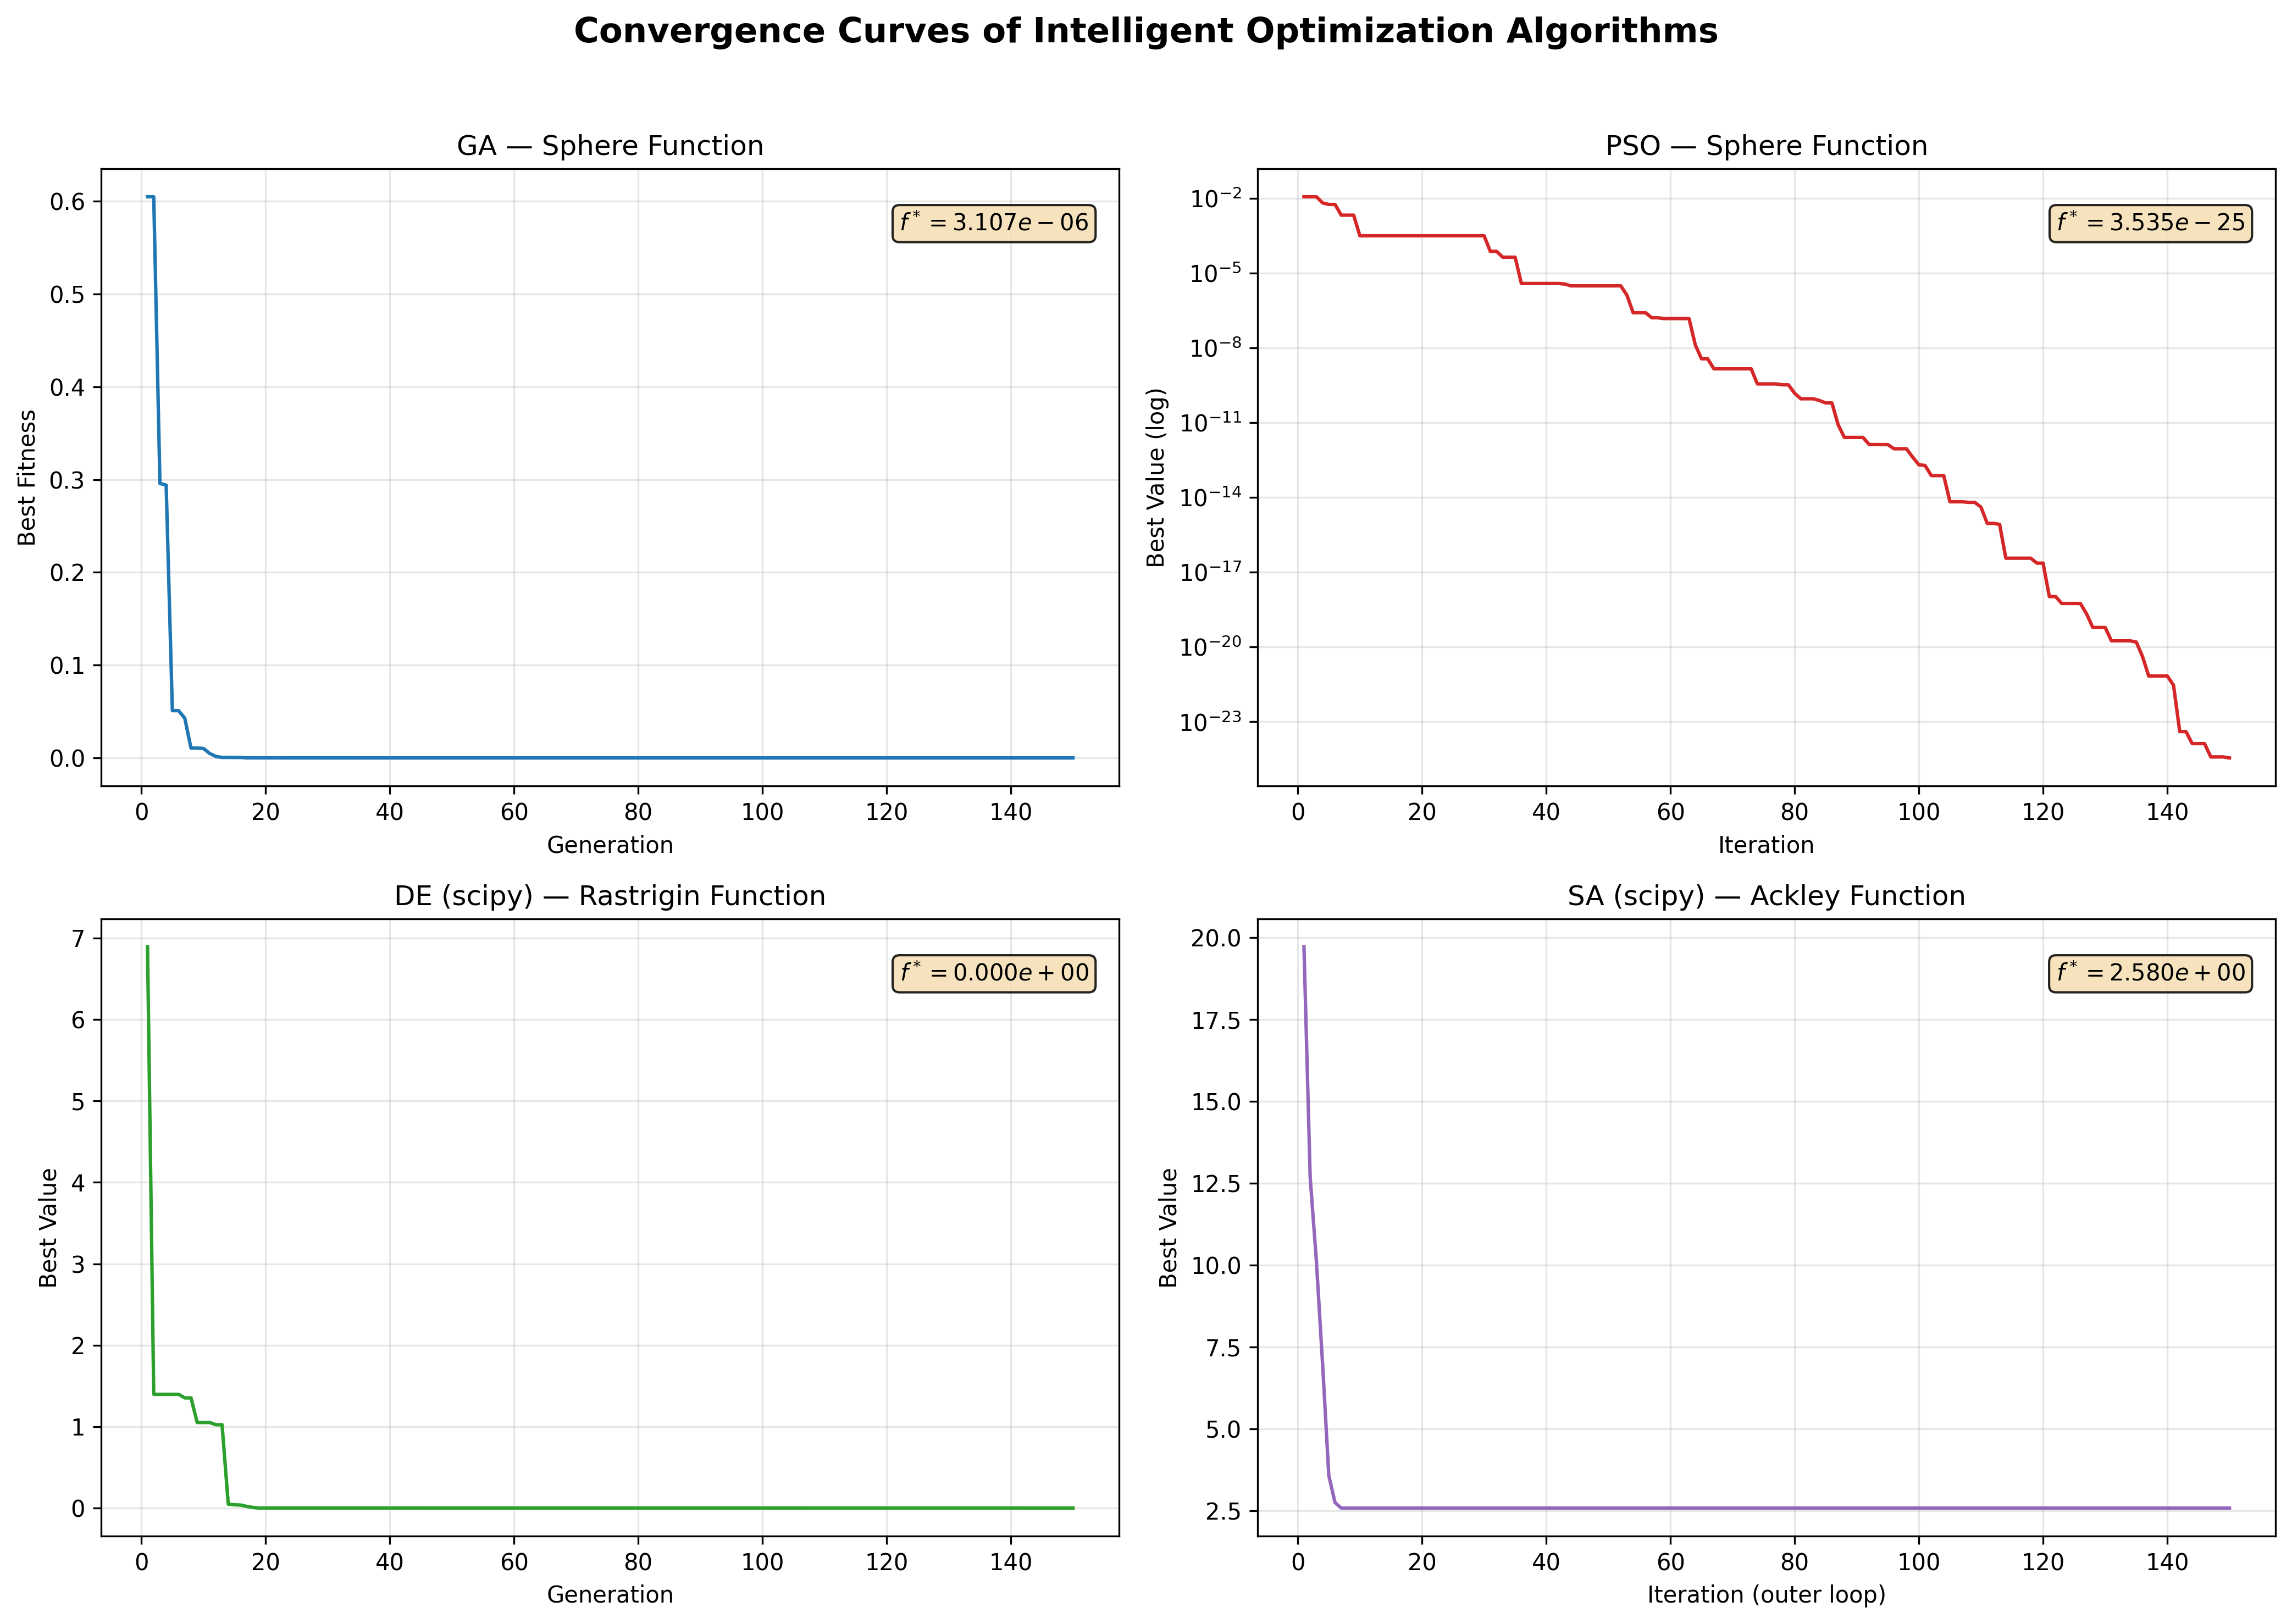
\includegraphics[width=\textwidth]{../output/intelligent_opt_result.png}
\caption{智能优化算法收敛曲线：GA（左上）、PSO（右上）、DE on Rastrigin（左下）、SA on Ackley（右下）}
\label{fig:intelligent_opt}
\end{figure}

% ============================================================
\section{生物种群与传染病模型}

种群动力学模型是微分方程建模的经典应用领域。从简单的指数增长到复杂的多物种相互作用，这些模型不仅适用于生物学，在经济学、流行病学、化学反应动力学中同样适用。

\subsection{从Malthus到Logistic}

Malthusian指数增长模型$\frac{dN}{dt}=rN$假设资源无限，预测种群无限增长。Logistic模型引入环境容纳量$K$：$\frac{dN}{dt}=rN(1-\frac{N}{K})$，当$N=K/2$时增长最快，$N\to K$时趋于饱和。

\subsection{传染病模型与R0}

SIR模型将人群分为易感者(S)、感染者(I)和康复者(R)三类。基本再生数$R_0=\beta/\gamma$是决定传染病是否爆发的最关键参数：$R_0<1$则疾病自然消亡，$R_0>1$则可能爆发。群体免疫阈值为$1-1/R_0$。本文对比了$R_0=0.8$、1.5、3.0、5.0四种情景的感染曲线，直观展示了$R_0$对疫情规模的决定性影响。

\subsection{捕食者-猎物模型}

Lotka-Volterra模型的相图分析揭示了捕食者与猎物之间的周期振荡关系——猎物先增长$\to$捕食者随之增长$\to$猎物被过度捕食而减少$\to$捕食者因食物减少而减少$\to$猎物恢复$\to$循环。这是一种结构性周期，不需要外部驱动。

\begin{figure}[htbp]
\centering
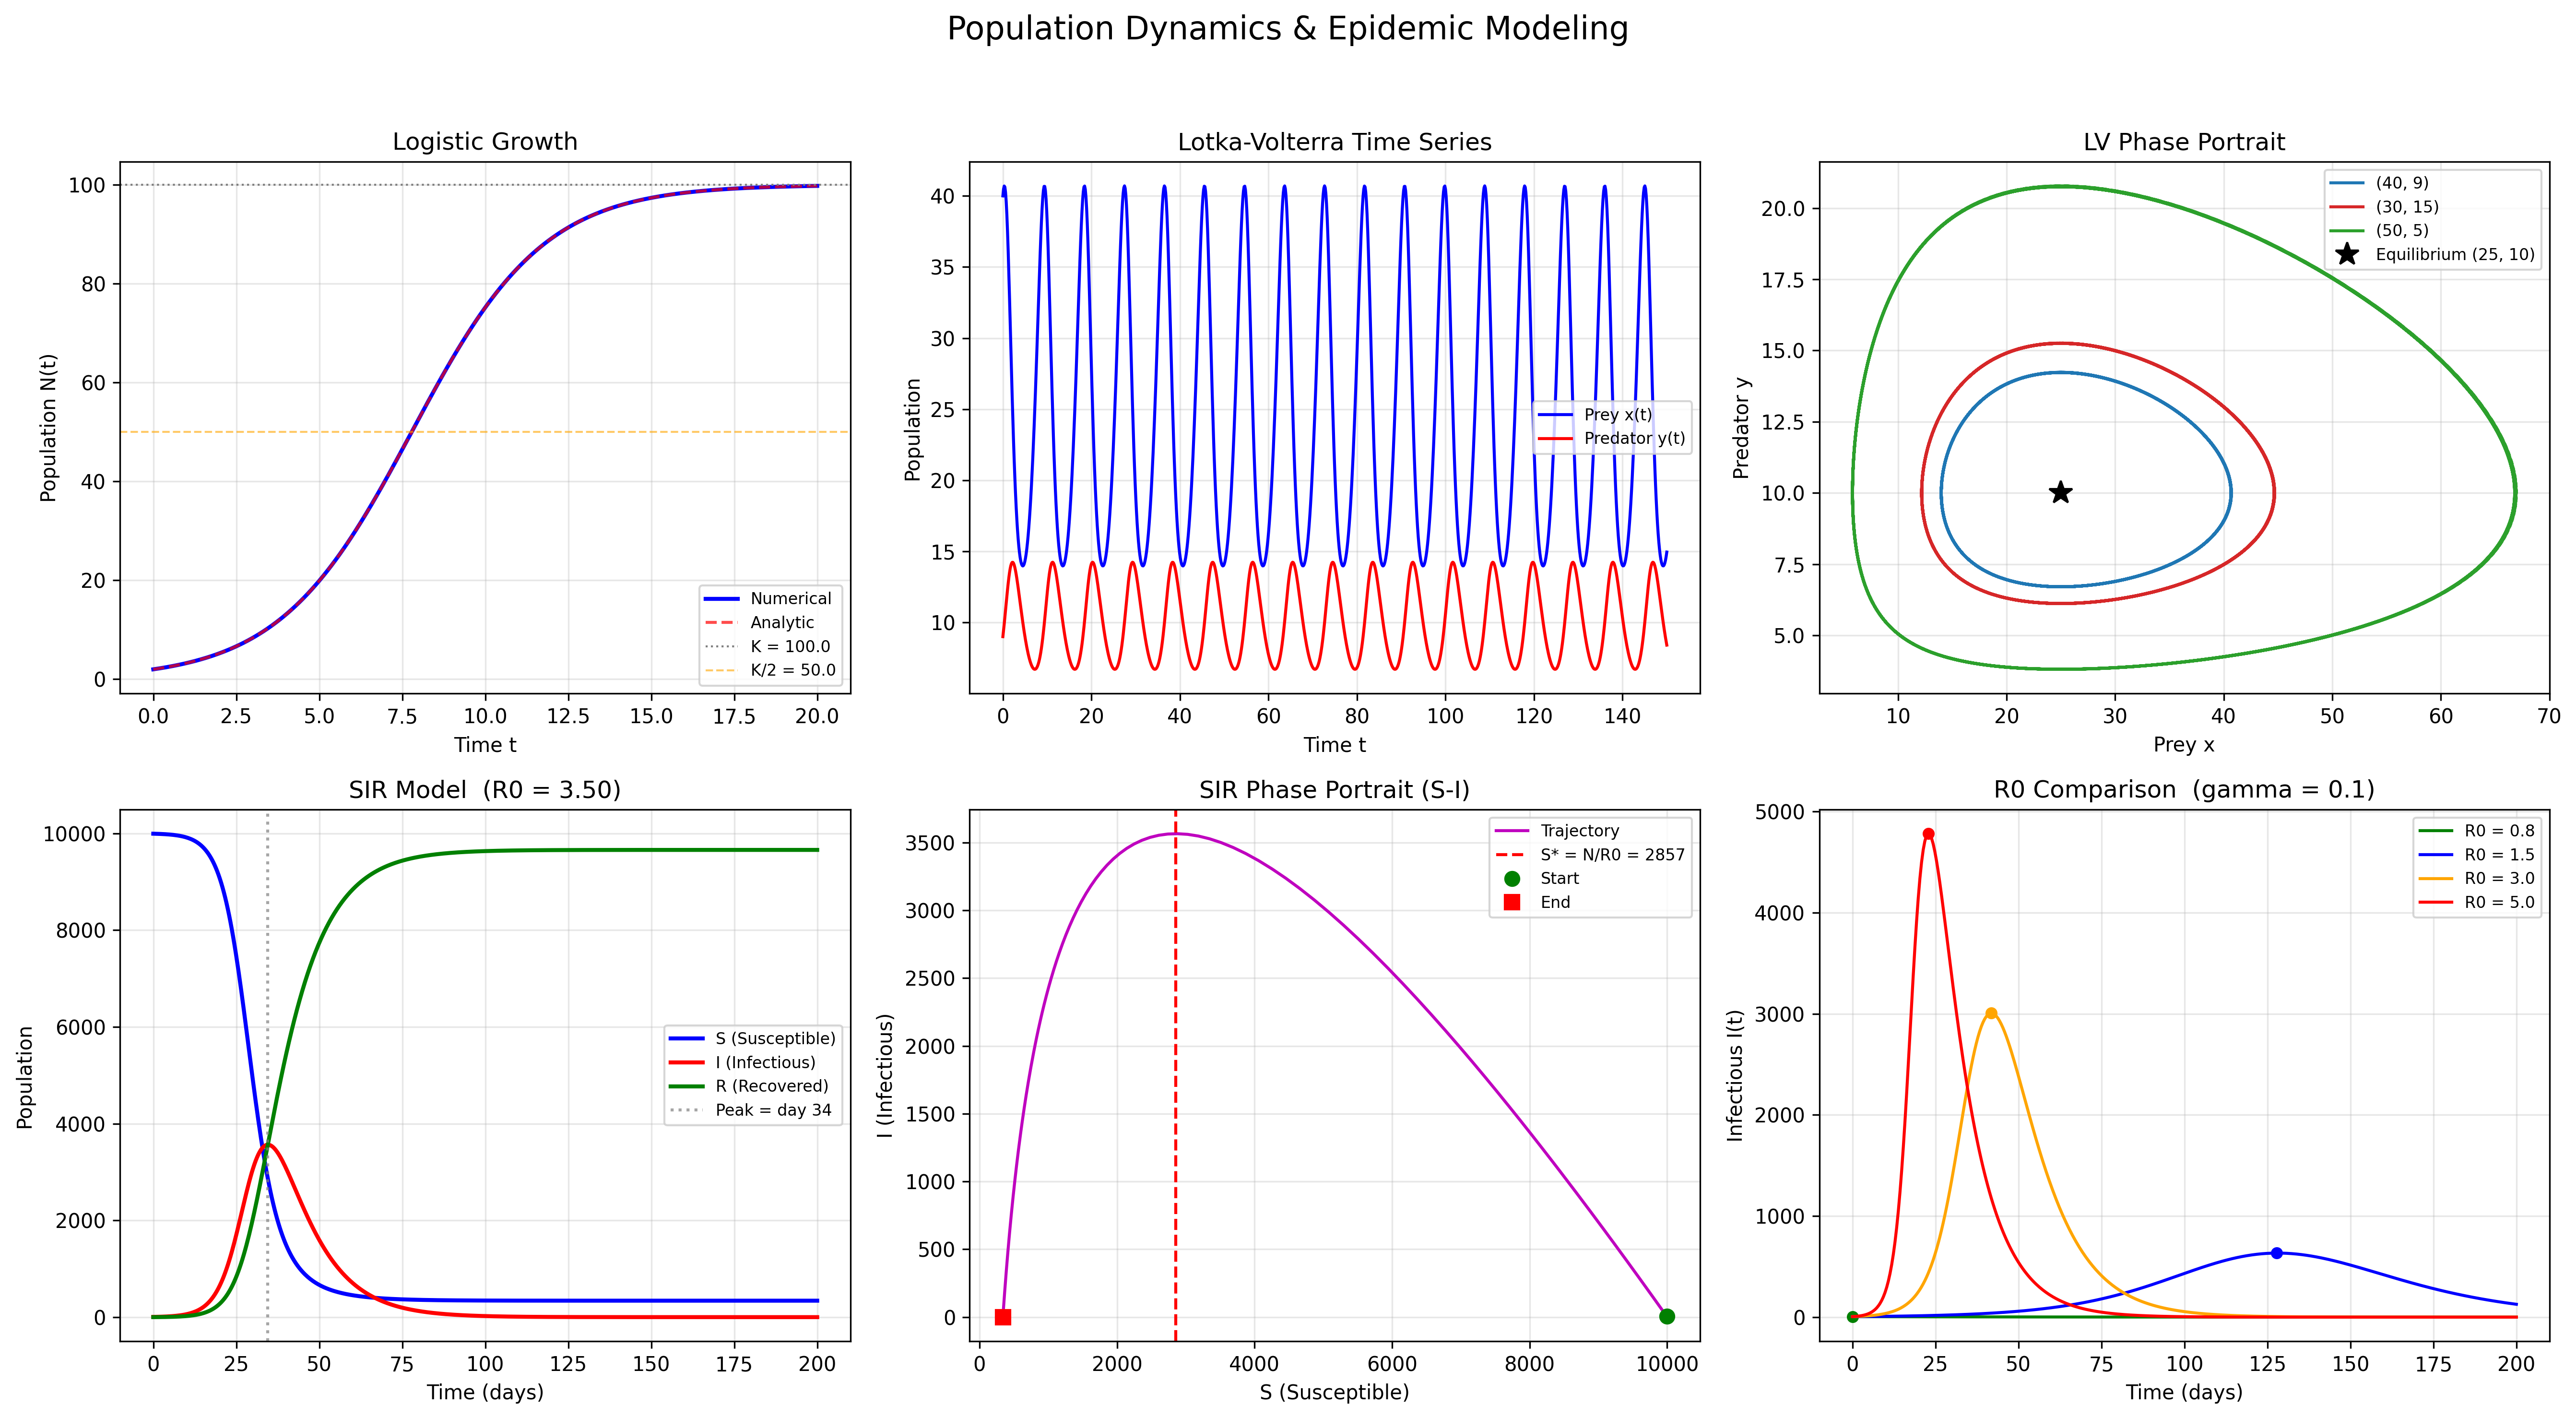
\includegraphics[width=\textwidth]{../output/population_result.png}
\caption{生物种群模型：Logistic增长（左上）、Lotka-Volterra时间序列（中上）、相图（右上）、SIR模型（左下）、SIR相平面（中下）、R0情景对比（右下）}
\label{fig:population}
\end{figure}

% ============================================================
\section{机器学习预测建模}

随着数据驱动建模在国赛中日益常见，掌握基本的机器学习方法成为编程手的必备技能。

\subsection{四种模型的对比}

本文使用合成的5特征数据集（其中2个为无关特征），对比了四种回归模型：
\begin{itemize}[nosep]
    \item \textbf{线性回归}：$R^2=0.9585$（最优），系数恢复最接近真实值。
    \item \textbf{岭回归 (Ridge)}：$R^2=0.9585$，通过L2正则化缓解多重共线性。
    \item \textbf{随机森林}：$R^2=0.9228$，对线性数据不如专用线性模型，但对非线性数据更鲁棒。
    \item \textbf{BP神经网络 (MLP)}：$R^2=0.9509$，适合复杂非线性映射。
\end{itemize}

\subsection{工程实践要点}

\begin{enumerate}[label=(\arabic*)]
    \item \textbf{数据划分}：坚持训练集/验证集/测试集三集拆分，在训练集上训练、验证集上调参、测试集上仅做最终评估。
    \item \textbf{特征缩放}：线性模型、神经网络对特征尺度敏感，必须标准化；树模型不受影响。
    \item \textbf{过拟合防治}：正则化（$L_1$/$L_2$）、早停(early stopping)、增加训练数据、降维。
    \item \textbf{国赛策略}：基线模型先用Ridge（简单可解释），主力模型用随机森林（鲁棒性好），提升模型用神经网络（复杂非线性），Lasso用于特征选择。
\end{enumerate}

\begin{figure}[htbp]
\centering
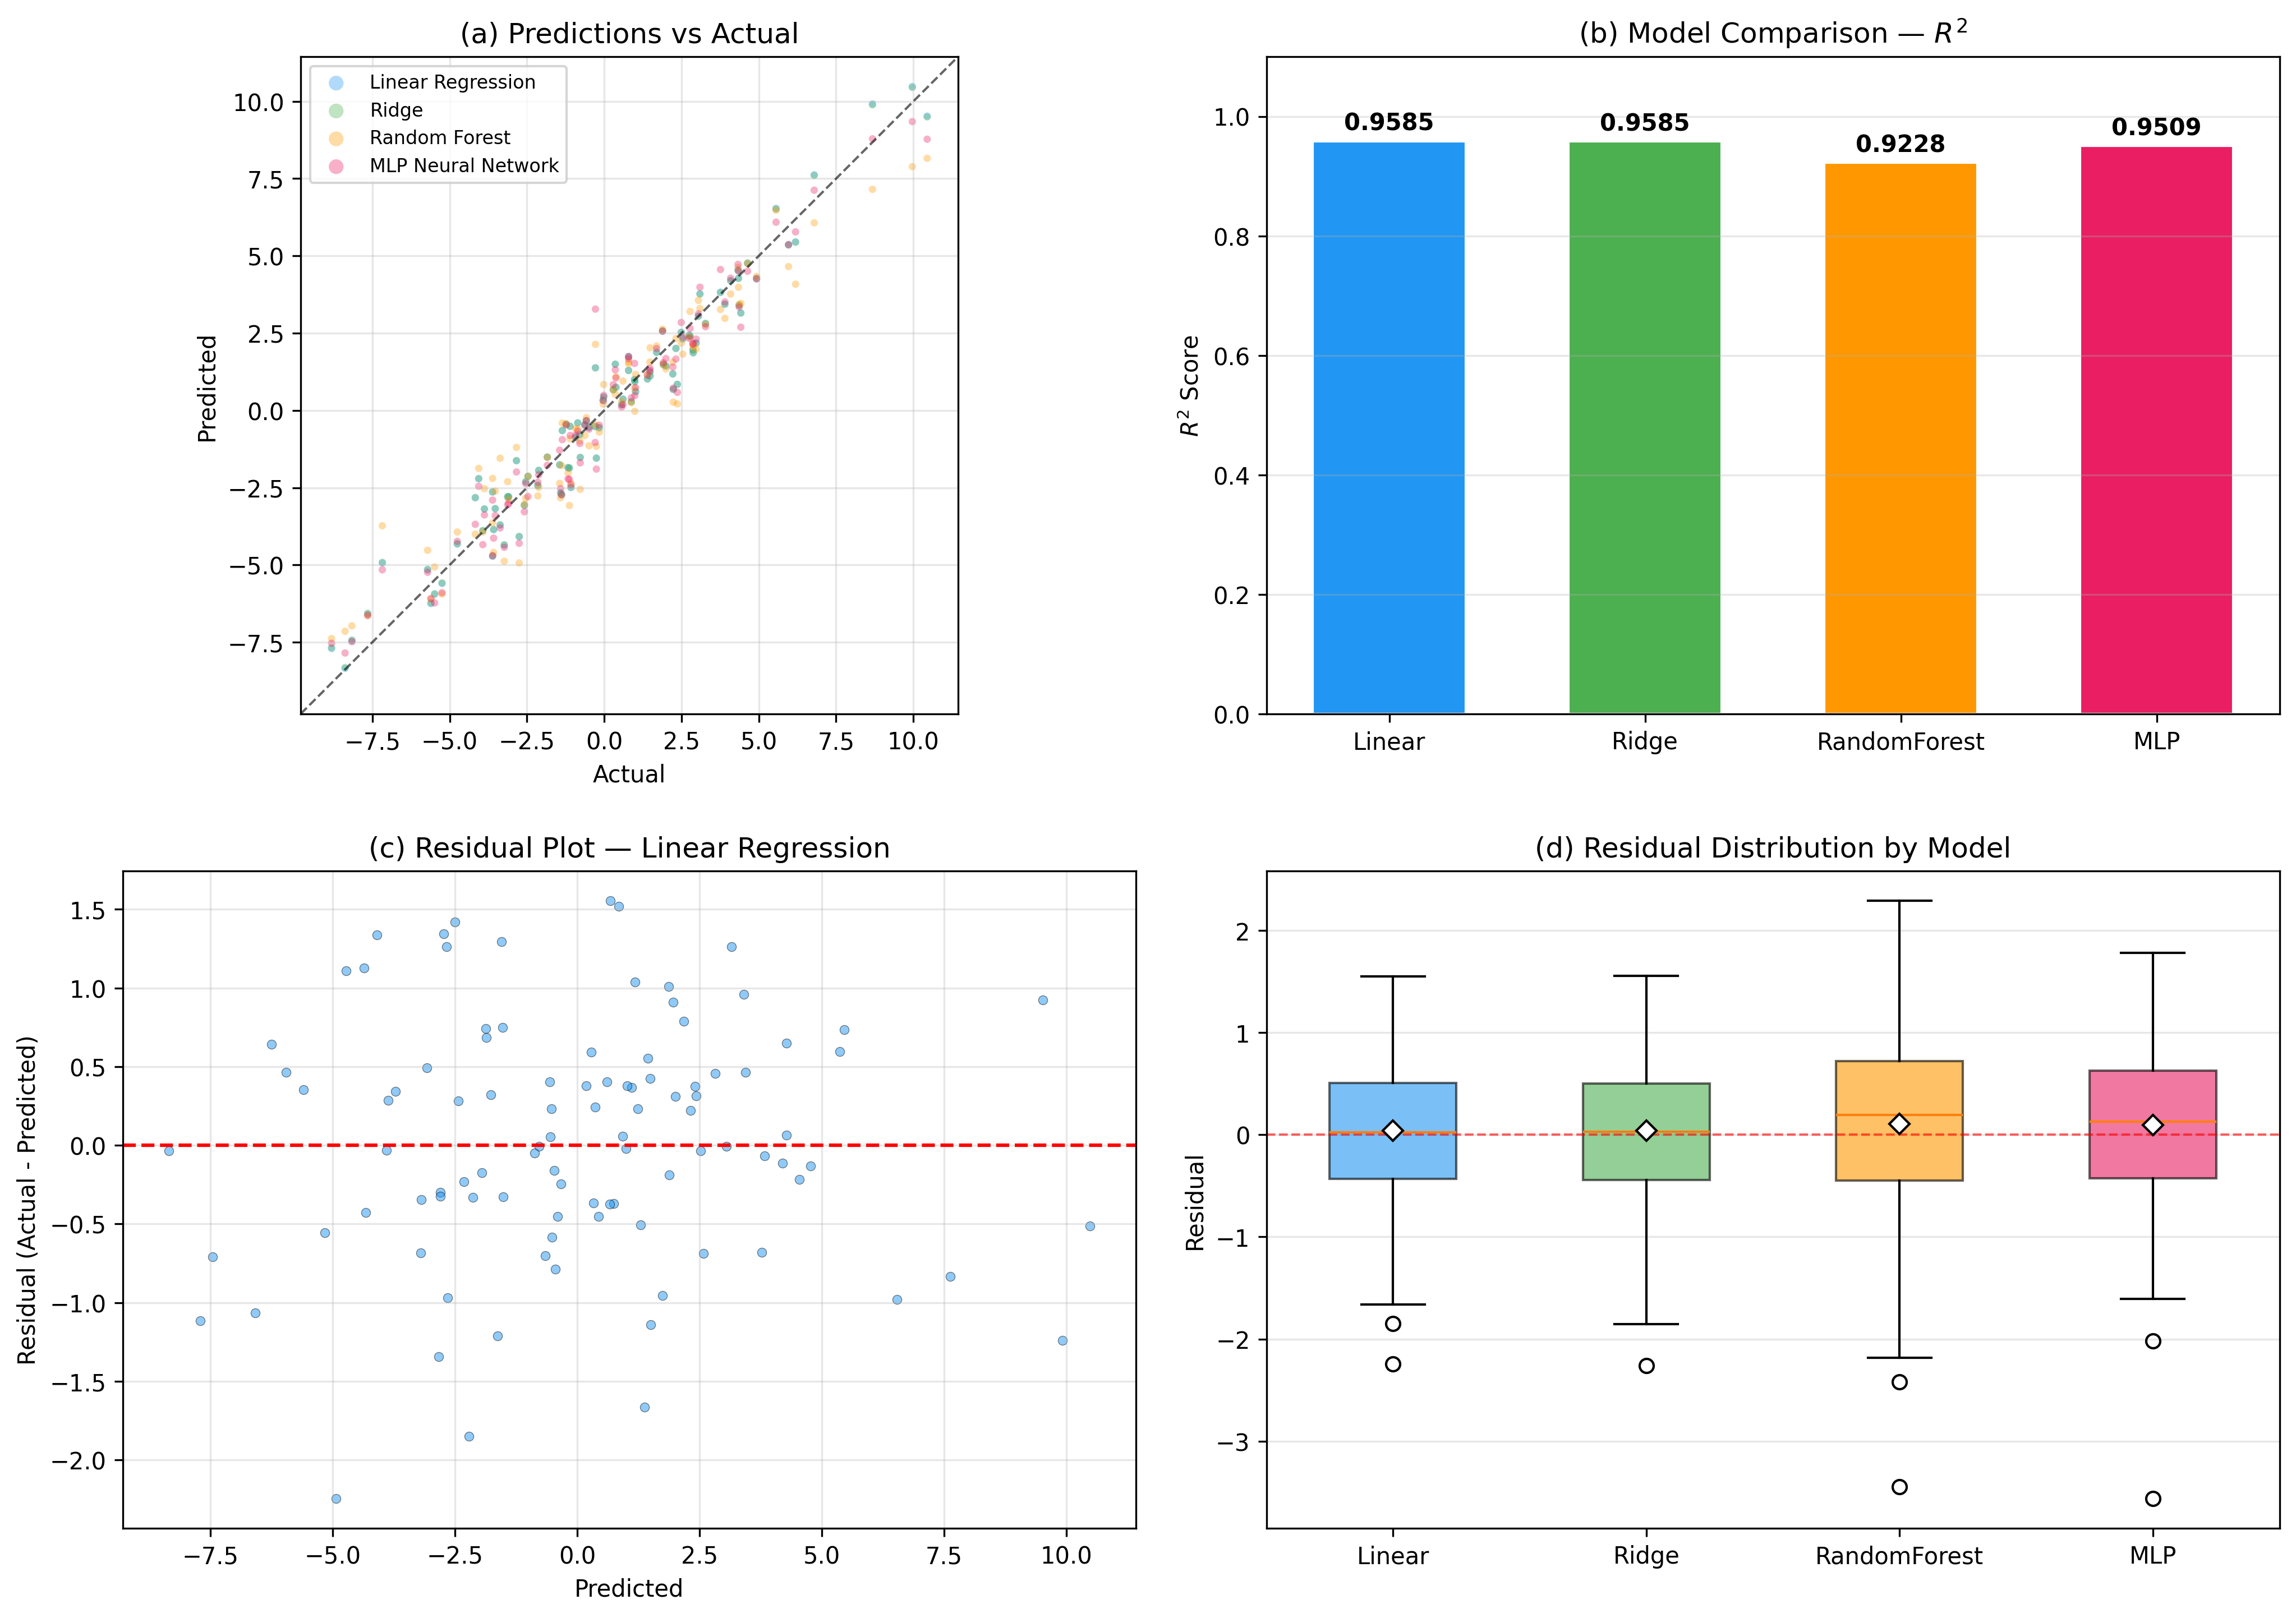
\includegraphics[width=\textwidth]{../output/ml_prediction_result.png}
\caption{机器学习预测模型对比：预测值vs真实值散点图（左上）、四模型R2得分对比（右上）、最优模型残差图（左下）、残差分布箱线图（右下）}
\label{fig:ml}
\end{figure}

% ============================================================
\section{计算电磁学：简化是核心}

电磁场相关的赛题在国赛中不常见，但出现就是区分度。面对复杂的Maxwell方程组，编程手的核心策略不是直接数值求解全耦合方程，而是根据物理条件做近似简化。

\subsection{三个层次的简化}

\begin{enumerate}[label=(\arabic*)]
    \item \textbf{低频+小尺寸} $\to$ 准静态近似，把场问题降维成Poisson/Laplace方程+电路等效。
    \item \textbf{高频+远场} $\to$ 射线模型，使用Friis传输方程：$L(d)=20\log_{10}(d)+20\log_{10}(f)-147.55$ (dB)。
    \item \textbf{传导+趋肤} $\to$ 趋肤深度公式$\delta=1/\sqrt{\pi f\mu_0\mu_r\sigma}$，结合传输线模型计算屏蔽效能。
\end{enumerate}

本文计算了8阵元均匀直线阵的远场方向图（极坐标+直角坐标dB表示），3dB波束宽度约25.6$^\circ$；绘制了2.4GHz信号在自由空间的路径损耗曲线（1m到1000m范围）；并对比了铜、铝、铁三种导体在10Hz至1GHz的趋肤深度变化。

\begin{figure}[htbp]
\centering
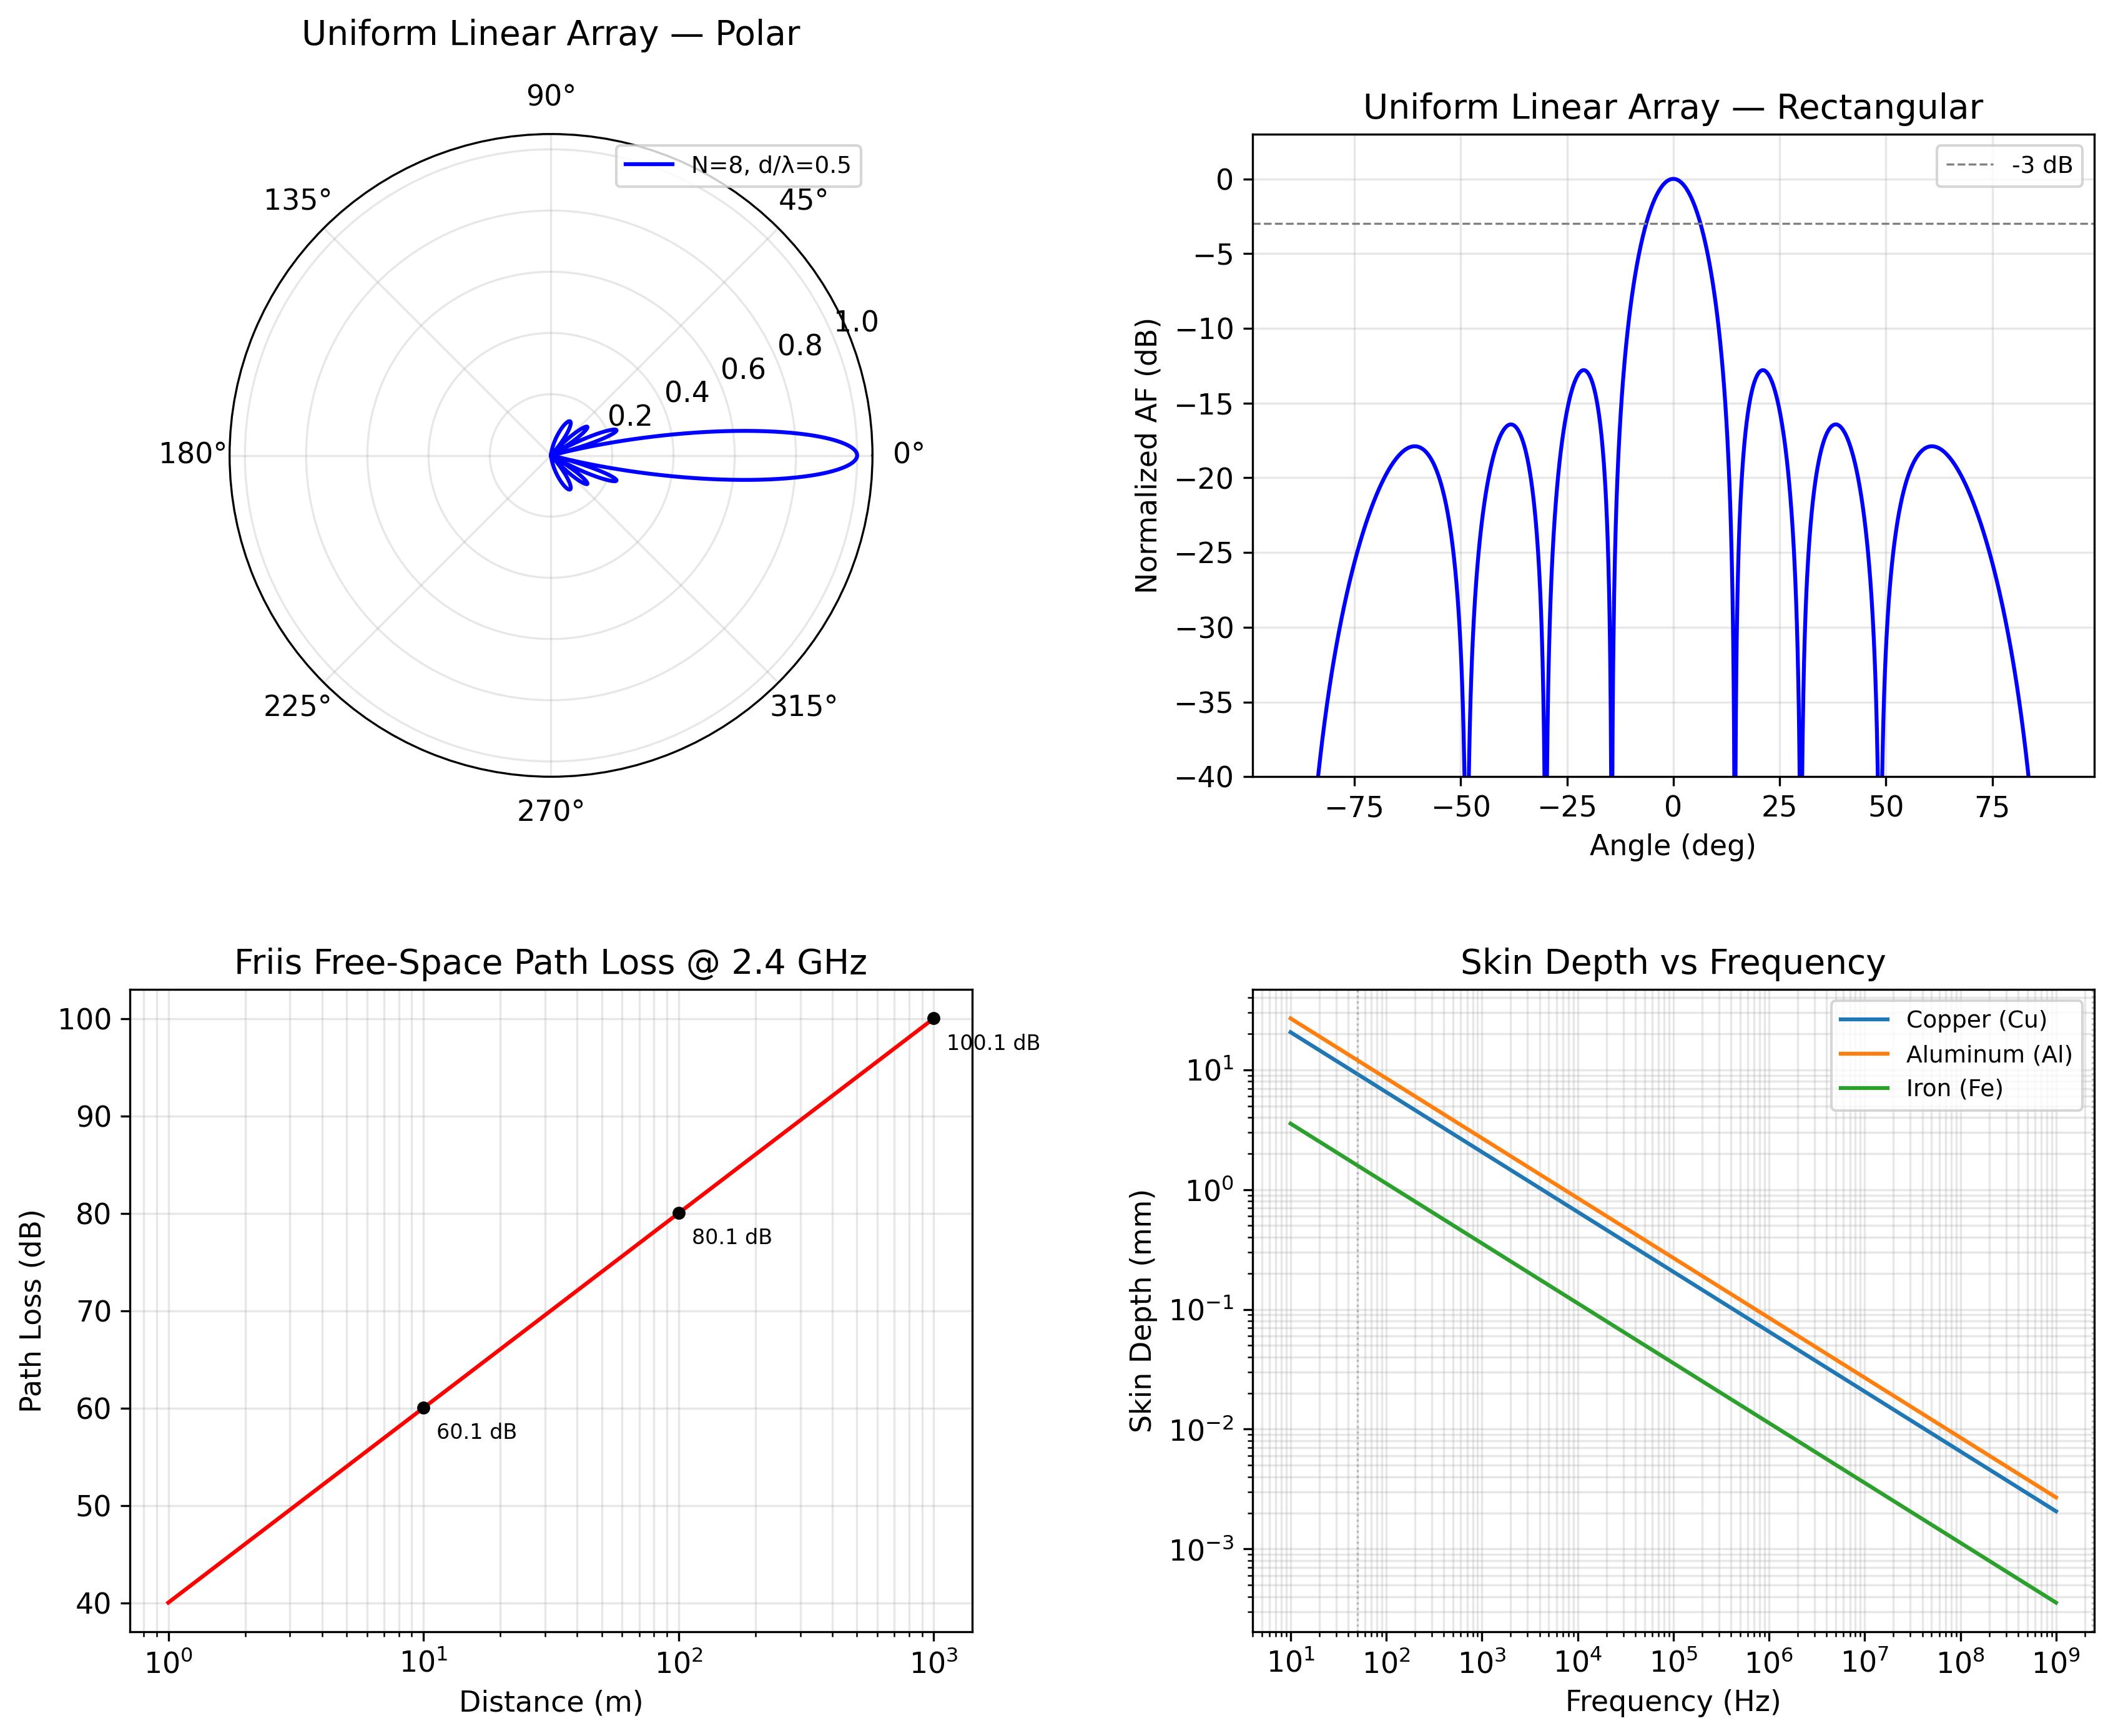
\includegraphics[width=\textwidth]{../output/electromagnetics_result.png}
\caption{计算电磁学演示：天线阵列方向图（左上极坐标、右上直角坐标）、Friis路径损耗（左下）、趋肤深度vs频率（右下）}
\label{fig:em}
\end{figure}

% ============================================================
\section{CT图像重建：从投影到图像}

2017年国赛A题``CT系统参数标定及成像''是一个经典的逆问题建模案例。其本质是将X射线不同角度下的投影数据（Radon变换），通过反演算法重建物体内部的衰减系数分布。

\subsection{Radon变换与FBP重建}

Radon变换的正问题是将二维图像沿各方向积分得到投影（正弦图）：
\begin{equation}
p(s,\theta) = \iint \mu(x,y)\;\delta(x\cos\theta+y\sin\theta - s)\;dx\,dy
\end{equation}

逆问题的求解采用滤波反投影(FBP)方法：先对每个角度的投影做傅里叶变换，在频域乘以斜坡滤波器$|\omega|$以消除模糊，再反变换回空域，最后沿入射方向反投影回图像空间。

本文使用10个椭圆的叠加构造了一个简化的Shepp-Logan数字体模（256$\times$256像素），计算其180角度下的Radon变换（正弦图），分别使用直接反投影和FBP进行重建。结果显示：
\begin{itemize}[nosep]
    \item 直接反投影：RMSE=0.2507，图像模糊，SNR仅0.10 dB。
    \item FBP（Ram-Lak滤波器）：RMSE=0.0540，图像清晰锐利，SNR提升至13.43 dB（+13.33 dB）。
\end{itemize}

这正是FBP方法的核心价值——通过频域斜坡滤波，补偿了反投影过程中的低频过增强效应。

\begin{figure}[htbp]
\centering
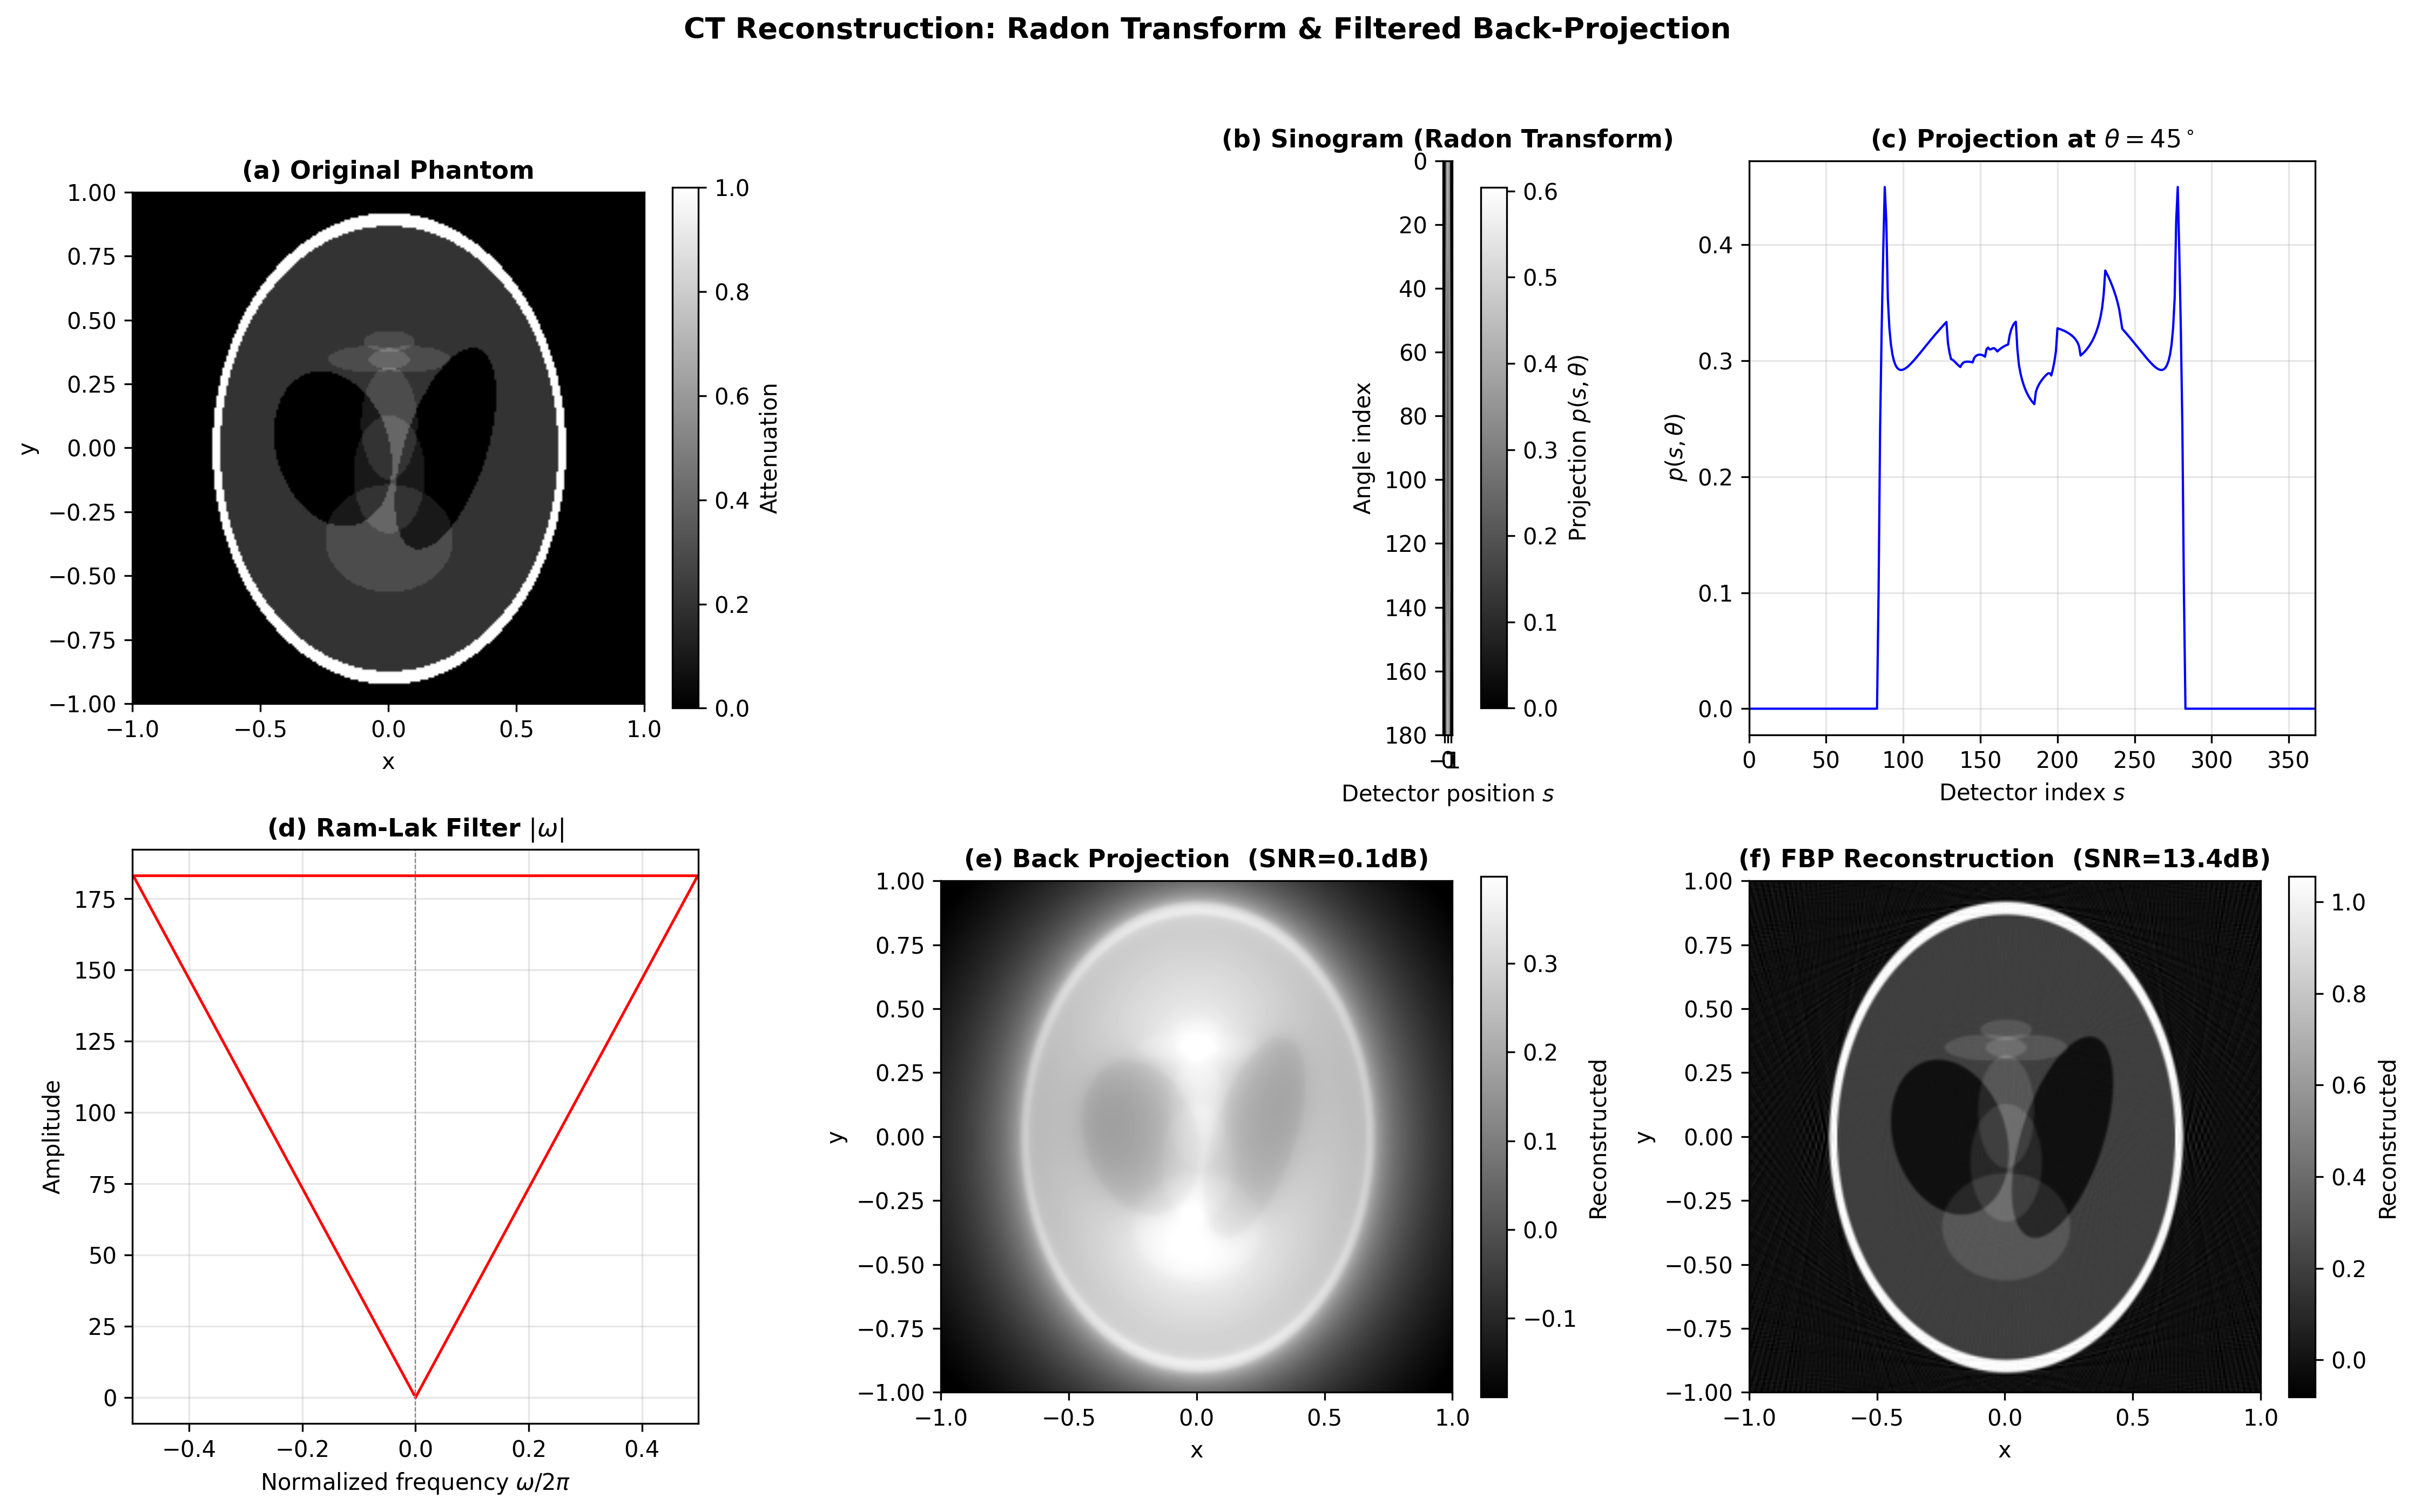
\includegraphics[width=\textwidth]{../output/ct_reconstruction_result.png}
\caption{CT图像重建：原始体模（左上）、正弦图（中上）、单角度投影曲线（右上）、Ram-Lak滤波器（左下）、直接反投影结果（中下）、FBP重建结果（右下）}
\label{fig:ct}
\end{figure}

% ============================================================
\section{总结与展望}

\subsection{方法体系总结}

本文系统梳理了十大建模方法模块，覆盖了国赛常见题型的核心技术需求：

\begin{table}[htbp]
\centering
\caption{十大方法模块与国赛题型对应关系}
\begin{tabular}{@{}llll@{}}
\toprule
\textbf{模块} & \textbf{核心方法} & \textbf{Python工具} & \textbf{对应题型} \\
\midrule
优化方法 & LP, IP, 0-1, MIP & SciPy, PuLP & 资源分配、生产计划 \\
图论算法 & Dijkstra, MST, MaxFlow & NetworkX & 交通、物流、通信 \\
微分方程 & ODE(P), PDE数值解 & SciPy(solve\_ivp) & 物理、生物、化学 \\
决策评价 & AHP, TOPSIS, 熵权法 & NumPy(自行实现) & 综合评价、方案比选 \\
插值拟合 & 样条插值, 最小二乘 & SciPy(interpolate) & 数据预处理 \\
智能优化 & GA, PSO, DE, SA & SciPy(optimize) & NP-hard、非凸问题 \\
生物种群 & Logistic, SIR, LV & SciPy(solve\_ivp) & 预测、流行病建模 \\
机器学习 & 线性/岭/RF/MLP & scikit-learn & 数据驱动预测 \\
电磁场 & Friis, 趋肤深度 & NumPy & 天线、屏蔽、无线充电 \\
CT重建 & Radon, FBP & NumPy, SciPy(fft) & 成像、反演、逆问题 \\
\bottomrule
\end{tabular}
\label{tab:summary}
\end{table}

\subsection{编程手的工作流}

在国赛72小时中，编程手应遵循以下工作流：收到建模手的模型方案后，\textbf{(1)}快速判断模型类型$\to$\textbf{(2)}从代码模板库中找到对应模板$\to$\textbf{(3)}修改参数和数据接口$\to$\textbf{(4)}运行并验证结果合理性$\to$\textbf{(5)}生成高清可视化图表供论文手使用。本文建立的10个demo脚本正是为此流程服务的代码模板库。

\subsection{后续计划}

第二阶段（8月12日至9月6日）将进行三轮专题实战训练（预测评价类、优化仿真类、综合创新类各一轮）。届时将利用本文建立的方法体系，在4天实战周期中快速响应各种题型，同时持续完善代码库和模板。

\begin{thebibliography}{9}
\bibitem{siyuan} 司守奎, 孙玺菁. 数学建模算法与应用(第3版). 国防工业出版社, 2023.
\bibitem{jiang} 姜启源, 谢金星, 叶俊. 数学模型(第5版). 高等教育出版社, 2018.
\bibitem{cumcm2017} 全国大学生数学建模竞赛组委会. 2017年高教社杯全国大学生数学建模竞赛A题: CT系统参数标定及成像.
\bibitem{scipy} Virtanen P, et al. SciPy 1.0: fundamental algorithms for scientific computing in Python. Nature Methods, 2020.
\bibitem{networkx} Hagberg A, et al. Exploring Network Structure, Dynamics, and Function using NetworkX. SciPy 2008.
\bibitem{sklearn} Pedregosa F, et al. Scikit-learn: Machine Learning in Python. JMLR, 2011.
\end{thebibliography}

\end{document}
